\documentclass[11pt,a4paper]{article}

% Image mode: pdf.
% Image paths stay relative. In PDF mode, place same-basename PDF conversions
% of the chapter SVG files in the assets/ directory beside this source.

\usepackage{iftex}
\ifPDFTeX
  \PackageError{handout}{This template requires XeTeX or Tectonic}{Compile with xelatex or tectonic.}
\fi

\usepackage[a4paper,top=18mm,bottom=20mm,left=20mm,right=20mm,headsep=6mm]{geometry}
\usepackage{fontspec}
\usepackage{xeCJK}
\usepackage{amsmath}
\usepackage{unicode-math}

% Font settings are intentionally visible in the generated .tex file.
% These defaults target the macOS machine used for the released PDF.
% Change the family names when compiling on another system.
\setmainfont{Songti TC}
\setsansfont{Heiti TC}
\setmonofont{Menlo}
\setCJKmainfont{Songti TC}
\setCJKsansfont{Heiti TC}
\setCJKmonofont{Heiti TC}
\setmathfont{STIX Two Math}
\XeTeXlinebreaklocale "zh"
\XeTeXlinebreakskip=0pt plus 1pt

\usepackage{xcolor}
\definecolor{HandoutBlue}{HTML}{215A91}
\definecolor{HandoutBlueLight}{HTML}{EEF5FC}
\definecolor{HandoutGreen}{HTML}{39715A}
\definecolor{HandoutGreenLight}{HTML}{EFF8F3}
\definecolor{HandoutGold}{HTML}{8A641C}
\definecolor{HandoutGoldLight}{HTML}{FFF8E8}
\definecolor{HandoutInk}{HTML}{253142}
\definecolor{HandoutMuted}{HTML}{667085}

\usepackage{graphicx}
\makeatletter
% Pandoc 3 emits an accessibility `alt` key for raster/PDF images. Older
% graphicx releases do not know that key, so accept it without changing layout.
\@ifundefined{KV@Gin@alt}{\define@key{Gin}{alt}{}}{}
\newsavebox\pandoc@box
\newcommand*\pandocbounded[1]{%
  \sbox\pandoc@box{#1}%
  \Gscale@div\@tempa{\textheight}{\dimexpr\ht\pandoc@box+\dp\pandoc@box\relax}%
  \Gscale@div\@tempb{\linewidth}{\wd\pandoc@box}%
  \ifdim\@tempb\p@<\@tempa\p@\let\@tempa\@tempb\fi
  \ifdim\@tempa\p@<\p@\scalebox{\@tempa}{\usebox\pandoc@box}%
  \else\usebox{\pandoc@box}%
  \fi
}
\makeatother
\usepackage{float}
\floatplacement{figure}{H}
% Pandoc uses LTcaptype=none for uncaptioned longtables. The caption package
% expects that name to exist as a counter even though it is never displayed.
\newcounter{none}
\usepackage{caption}
\captionsetup[figure]{labelformat=empty,labelsep=none,font=small}

\usepackage{booktabs,longtable,array,calc}
\usepackage{etoolbox}
\makeatletter
\patchcmd\longtable{\par}{\if@noskipsec\mbox{}\fi\par}{}{}
\makeatother

\usepackage[most]{tcolorbox}
\tcbuselibrary{breakable,skins}
\newtcolorbox{HandoutLearningMap}{
  enhanced,breakable,colback=HandoutBlueLight,colframe=HandoutBlue,
  boxrule=0.8pt,arc=1.5mm,left=3mm,right=3mm,top=2mm,bottom=2mm,
  before skip=8pt,after skip=10pt
}
\newtcolorbox{HandoutWorkedExample}{
  enhanced,breakable,colback=HandoutGreenLight,colframe=HandoutGreen,
  boxrule=0.65pt,arc=1.5mm,left=3mm,right=3mm,top=2mm,bottom=2mm,
  before skip=8pt,after skip=10pt
}
\newtcolorbox{HandoutSelfCheck}{
  enhanced,breakable,colback=HandoutGoldLight,colframe=HandoutGold,
  boxrule=0.65pt,arc=1.5mm,left=3mm,right=3mm,top=2mm,bottom=2mm,
  before skip=8pt,after skip=10pt
}

\usepackage{titlesec}
\titleformat{\section}{\sffamily\bfseries\Large\color{HandoutBlue}}{}{0pt}{}
\titleformat{\subsection}{\sffamily\bfseries\large\color{HandoutInk}}{}{0pt}{}
\titleformat{\subsubsection}{\sffamily\bfseries\normalsize\color{HandoutInk}}{}{0pt}{}
\titlespacing*{\section}{0pt}{1.4em}{0.55em}
\titlespacing*{\subsection}{0pt}{1.15em}{0.45em}
\titlespacing*{\subsubsection}{0pt}{0.9em}{0.35em}
\setcounter{secnumdepth}{-\maxdimen}

\usepackage{hyperref}
\usepackage{bookmark}
\IfFileExists{xurl.sty}{\usepackage{xurl}}{}
\urlstyle{same}
\hypersetup{
  colorlinks=true,
  linkcolor=HandoutBlue,
  urlcolor=HandoutBlue,
  citecolor=HandoutBlue,
  pdftitle={選物I-4 牛頓運動定律},
  pdfsubject={物理},
  pdfcreator={Pandoc with the HighSchooContent LaTeX template}
}

\setlength{\parindent}{0pt}
\setlength{\parskip}{0.55em plus 0.15em minus 0.1em}
\setlength{\emergencystretch}{3em}
\setlength{\LTpre}{0.5em}
\setlength{\LTpost}{0.5em}
\renewcommand{\arraystretch}{1.18}
\providecommand{\tightlist}{%
  \setlength{\itemsep}{0pt}\setlength{\parskip}{0pt}}
\pagestyle{plain}


\begin{document}

\begin{tcolorbox}[
  enhanced,colback=white,colframe=HandoutBlue,boxrule=1.1pt,arc=2mm,
  borderline west={3pt}{0pt}{HandoutBlue},left=5mm,right=4mm,top=4mm,bottom=4mm
]
{\sffamily\small\bfseries\color{HandoutBlue}學生講義}\par
{\sffamily\bfseries\LARGE\color{HandoutInk}選物I-4 牛頓運動定律}\par
\vspace{0.35em}{\large 從運動描述連結受力、圓周與振盪}\par
\vspace{0.45em}{\small\color{HandoutMuted}%
科目：物理
\quad 課程：普通高中選修物理 I
\quad 版本：學生版｜核心＋理解
\quad 校訂：2026-08-29
}\par
\vspace{0.25em}{\small\color{HandoutMuted}範圍：現行選修主線；含等速圓周與簡諧運動}\par
\end{tcolorbox}


\begin{HandoutLearningMap}

\subsection{本章核心關係}\label{ux672cux7ae0ux6838ux5fc3ux95dcux4fc2}

\begin{enumerate}
\def\labelenumi{\arabic{enumi}.}
\tightlist
\item
  \textbf{力為什麼一定是向量？}──同樣大小、不同方向會造成不同加速度；多個力要以分量合成。
\item
  \textbf{沒有合力時，物體為什麼不需要「維持運動的力」？}──牛頓第一定律說它會維持靜止或等速度直線運動。
\item
  \textbf{\(\sum\vec F=m\vec a\) 計算什麼？}──同一受力體上所有外力的向量和，決定它的加速度。
\item
  \textbf{作用力與反作用力為什麼不互相抵銷？}──兩力作用在不同物體；只有同一物體上的力才能相加。
\item
  \textbf{圓周運動速率不變，為什麼仍需合力？}──速度方向持續改變，向心加速度必指向圓心。
\item
  \textbf{彈簧為什麼會來回？sin、cos 又從哪裡來？}──回復力 \(-kx\) 讓 \(a=-\omega^2x\)；這正是等速圓周投影的分量關係。
\item
  \textbf{實務上用在哪裡？}──機器人控制、秤重、電梯安全、彎道設計、離心設備與手機微型感測器，都在把「力---加速度---位移」串成可預測模型。
\end{enumerate}

{藍色：114 第 4 章核心}
{青綠：理解與應用}
{紫色：教材探索／延伸}

\end{HandoutLearningMap}

\section{Part A｜從受力圖到牛頓定律}\label{part-aux5f9eux53d7ux529bux5716ux5230ux725bux9813ux5b9aux5f8b}

\section{0. 自由體圖以受力體為中心}\label{ux81eaux7531ux9ad4ux5716ux4ee5ux53d7ux529bux9ad4ux70baux4e2dux5fc3}

一句「繩子有拉力」資訊不足。要說清楚：\textbf{誰作用在誰上、方向如何}。本章所有方程都要先選一個受力體；\(\sum\vec F\) 只收集外界作用在這個受力體上的力。

\begin{figure}
\centering
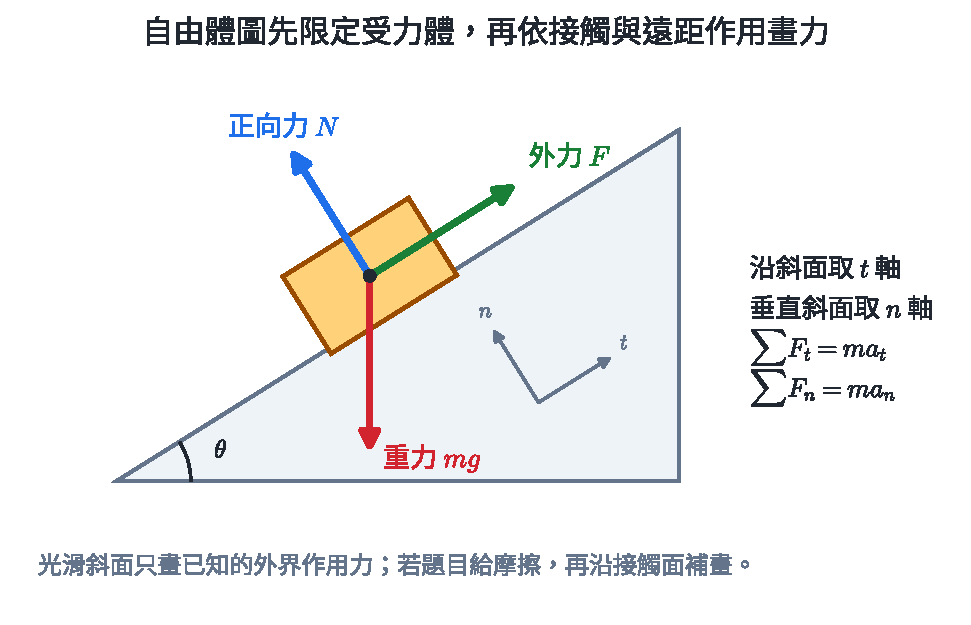
\includegraphics[width=0.94\linewidth,height=\textheight,keepaspectratio,alt={圖 0｜黃色物塊是受力體；重力、正向力與外力的箭頭都由物塊出發，斜面座標軸與後續分量方程對齊。}]{assets/選物I-4-受力圖.pdf}
\caption{圖 0｜黃色物塊是受力體；重力、正向力與外力的箭頭都由物塊出發，斜面座標軸與後續分量方程對齊。}
\end{figure}

自由體圖的固定操作是：

\begin{enumerate}
\def\labelenumi{\arabic{enumi}.}
\tightlist
\item
  圈定受力體；
\item
  由周遭的施力者找到接觸力與遠距力；
\item
  每一支力標示方向與符號；
\item
  選擇與加速度或接觸面對齊的座標軸；
\item
  逐軸將圖上的力收入 \(\sum F=ma\)。
\end{enumerate}

\begin{HandoutWorkedExample}

\subsection{完整示範｜書靜止在桌上並受水平拉力}\label{ux5b8cux6574ux793aux7bc4ux66f8ux975cux6b62ux5728ux684cux4e0aux4e26ux53d7ux6c34ux5e73ux62c9ux529b}

以書為受力體。人向右拉書，書仍靜止，圖上有地球對書的重力 \(mg\)、桌面對書的正向力 \(N\)、人對書的拉力 \(F\) 與桌面對書的靜摩擦力 \(f_s\)。

書的加速度為 0，因此

\[
N-mg=0,
\qquad
F-f_s=0.
\]

本題得到 \(N=mg\)、\(f_s=F\) 是平衡條件的結果。若拉力有向上分量，\(N\) 會跟著改變。

\end{HandoutWorkedExample}

\begin{HandoutWorkedExample}

\subsection{完整示範｜吊燈的力與第三定律力對}\label{ux5b8cux6574ux793aux7bc4ux540aux71c8ux7684ux529bux8207ux7b2cux4e09ux5b9aux5f8bux529bux5c0d}

吊燈靜止懸掛在繩下。以吊燈為受力體，只畫地球對燈的重力 \(mg\) 向下與繩對燈的張力 \(T\) 向上。

\[
T-mg=0
\quad\Rightarrow\quad
T=mg.
\]

燈對繩的力作用在繩上，它與繩對燈的力是第三定律力對，分屬兩張自由體圖。

\end{HandoutWorkedExample}

\begin{HandoutSelfCheck}

\subsection{練習｜自由體圖的 4 種情境}\label{ux7df4ux7fd2ux81eaux7531ux9ad4ux5716ux7684-4-ux7a2eux60c5ux5883}

\begin{enumerate}
\def\labelenumi{\arabic{enumi}.}
\tightlist
\item
  蘋果離手後在空中落下，忽略空氣阻力。列出蘋果的受力。
\item
  人站在靜止電梯地板上。列出人的受力。
\item
  物塊在光滑斜面上下滑。列出真實力，再選擇座標軸。
\item
  小球由水平繩子拉著繞圓，忽略其他水平作用。列出水平面內的力與方向。
\end{enumerate}

\textbf{簡答：}1. 只有地球對蘋果的重力向下。2. 重力向下、地板正向力向上。3. 重力與正向力；座標取沿斜面與垂直斜面。4. 繩張力指向圓心。

\end{HandoutSelfCheck}

\begin{HandoutSelfCheck}

\subsection{練習}\label{ux7df4ux7fd2}

手向右推箱子。畫箱子的自由體圖時，應畫「箱子推手的力」嗎？

\textbf{答案：}不畫。受力體是箱子，只畫手作用在箱子上的推力，以及地球、地面等外界作用在箱子上的力。箱子推手的力作用在手上。

\end{HandoutSelfCheck}

\section{1. 力的向量性與虎克定律}\label{ux529bux7684ux5411ux91cfux6027ux8207ux864eux514bux5b9aux5f8b}

力可以來自接觸，例如正向力、張力、彈力與摩擦作用；也可以不接觸，例如重力。力的 SI 單位是牛頓：

\[
1\ \mathrm N=1\ \mathrm{kg\,m/s^2}.
\]

若力 \(\vec F\) 與 \(+x\) 軸夾角為 \(\theta\)：

\[
F_x=F\cos\theta,
\qquad
F_y=F\sin\theta.
\]

多個力的合力為向量和：

\[
\vec F_{\text{net}}=\sum_i\vec F_i,
\qquad
F_{\text{net},x}=\sum_iF_{i,x},
\quad
F_{\text{net},y}=\sum_iF_{i,y}.
\]

\begin{HandoutWorkedExample}

\subsection{完整示範｜二維合力的分量、量值與方向}\label{ux5b8cux6574ux793aux7bc4ux4e8cux7dadux5408ux529bux7684ux5206ux91cfux91cfux503cux8207ux65b9ux5411}

一物體受 \(12\ \mathrm N\)、東偏北 \(30^\circ\) 的力，另受 \(5.0\ \mathrm N\) 向西。取東、北為正：

\[
F_x=12\cos30^\circ-5
=6\sqrt3-5
\approx5.39\ \mathrm N,
\]

\[
F_y=12\sin30^\circ=6.00\ \mathrm N.
\]

\[
F_{\mathrm{net}}=\sqrt{F_x^2+F_y^2}
\approx8.07\ \mathrm N,
\]

\[
\phi=\tan^{-1}\!\left(\frac{F_y}{F_x}\right)
\approx48.0^\circ.
\]

合力方向為東偏北 \(48.0^\circ\)。分量的正負由座標軸決定，量值保持為正。

\end{HandoutWorkedExample}

\subsection{彈簧的回復力}\label{ux5f48ux7c27ux7684ux56deux5fa9ux529b}

\begin{figure}
\centering
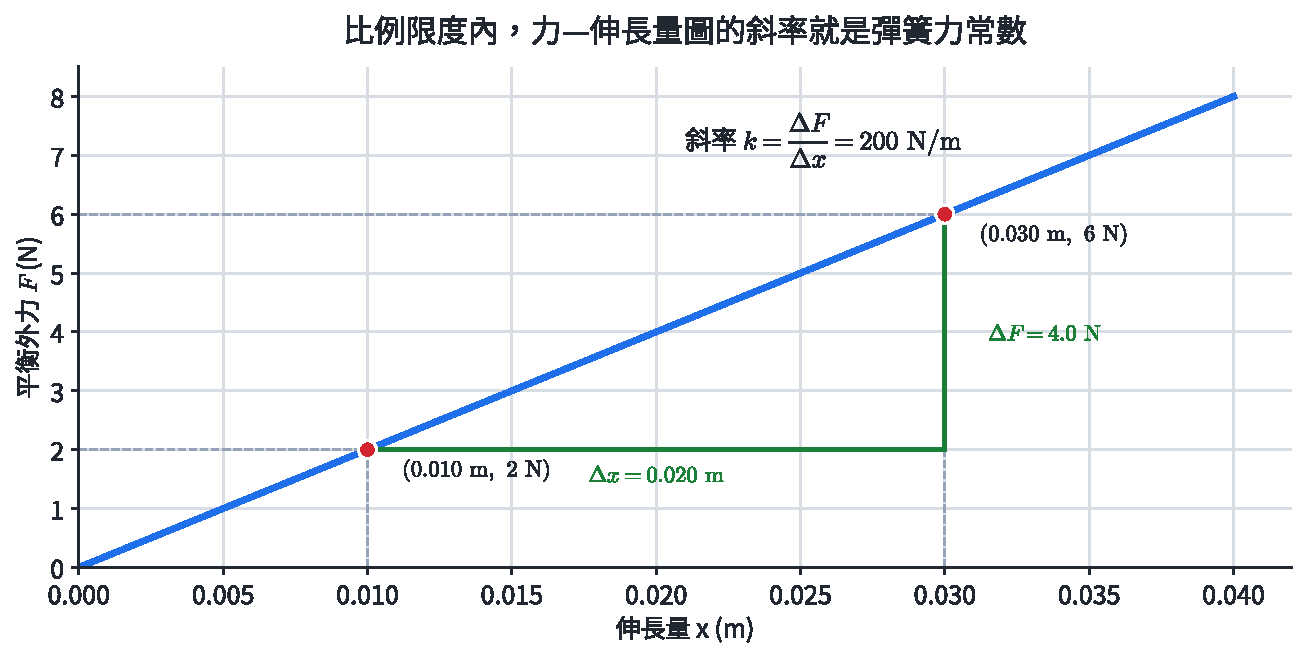
\includegraphics[width=0.92\linewidth,height=\textheight,keepaspectratio,alt={圖 1｜比例限度內，平衡外力與伸長量落在同一直線；圖上的斜率 \textbackslash Delta F/\textbackslash Delta x 等於彈簧力常數 k。}]{assets/選物I-4-虎克定律斜率.pdf}
\caption{圖 1｜比例限度內，平衡外力與伸長量落在同一直線；圖上的斜率 \(\Delta F/\Delta x\) 等於彈簧力常數 \(k\)。}
\end{figure}

圖 1 的兩點 \((0.010\ \mathrm m,2.0\ \mathrm N)\) 與 \((0.030\ \mathrm m,6.0\ \mathrm N)\) 給出同一斜率 \(k=200\ \mathrm{N/m}\)，因此校準後可由伸長量反推力。

在彈性比例限度內，理想彈簧的回復力遵守虎克定律：

\[
\boxed{\vec F_s=-k\vec x}.
\]

\(\vec x\) 是相對自然長度的形變；\(k\) 是力常數，SI 單位 \(\mathrm{N/m}\)。負號表示力與形變方向相反。若只問量值，才寫 \(F_s=k|x|\)。

比例限度之外，彈簧可能不再線性甚至永久變形，不能把 \(F=kx\) 無限延長。

\begin{HandoutWorkedExample}

\subsection{完整示範｜用斜率校準彈簧秤}\label{ux5b8cux6574ux793aux7bc4ux7528ux659cux7387ux6821ux6e96ux5f48ux7c27ux79e4}

在比例限度內，施力 \(2.0\ \mathrm N\) 時伸長 \(1.0\ \mathrm{cm}\)，故

\[
k=\frac{F}{x}=\frac{2.0}{0.010}=200\ \mathrm{N/m}.
\]

伸長 \(3.0\ \mathrm{cm}\) 時，回復力量值為 \((200)(0.030)=6.0\ \mathrm N\)，方向指向自然長度位置。

\end{HandoutWorkedExample}

\subsection{彈簧形變可轉換為重量讀數}\label{ux5f48ux7c27ux5f62ux8b8aux53efux8f49ux63dbux70baux91cdux91cfux8b80ux6578}

比例限度內 \(F=kx\)，量到彈簧位移即可反推力。實際 \(k\) 受材料、幾何與溫度影響，因此刻度須以已知力校準。超過比例限度後，力與形變不再維持同一斜率，甚至留下永久變形；原刻度隨之失效。

\begin{HandoutSelfCheck}

\subsection{練習}\label{ux7df4ux7fd2-1}

彈簧被向左壓縮 \(0.020\ \mathrm m\)，取向右為正，\(k=150\ \mathrm{N/m}\)。\(x\) 與彈簧力各為何？

\textbf{答案：}\(x=-0.020\ \mathrm m\)，\(F_s=-kx=+3.0\ \mathrm N\)，向右指向平衡位置。

\end{HandoutSelfCheck}

\begin{HandoutWorkedExample}

\subsection{完整示範｜由兩點校準彈簧並判斷比例限度}\label{ux5b8cux6574ux793aux7bc4ux7531ux5169ux9edeux6821ux6e96ux5f48ux7c27ux4e26ux5224ux65b7ux6bd4ux4f8bux9650ux5ea6}

平衡外力---伸長量圖在線性區通過 \((0.010\ \mathrm m,1.8\ \mathrm N)\) 與 \((0.040\ \mathrm m,7.2\ \mathrm N)\)。斜率為

\[
k=\frac{7.2-1.8}{0.040-0.010}
=180\ \mathrm{N/m}.
\]

在這條直線模型中，伸長 \(0.025\ \mathrm m\) 對應的平衡外力為

\[
F=kx=(180)(0.025)=4.5\ \mathrm N.
\]

若實測 \(x=0.055\ \mathrm m\) 時只需 \(8.0\ \mathrm N\)，而直線外推預測 \(9.9\ \mathrm N\)，實測點已偏離原斜率，該條線性校準的適用區間必須終止於更小形變。

\end{HandoutWorkedExample}

\begin{HandoutSelfCheck}

\subsection{練習｜向量力與虎克定律}\label{ux7df4ux7fd2ux5411ux91cfux529bux8207ux864eux514bux5b9aux5f8b}

\begin{enumerate}
\def\labelenumi{\arabic{enumi}.}
\tightlist
\item
  \(10\ \mathrm N\) 力向西偏北 \(37^\circ\)，求東、北分量。取 \(\sin37^\circ=0.6\)、\(\cos37^\circ=0.8\)。
\item
  一物體受 \((6,-8)\ \mathrm N\) 與 \((-2,5)\ \mathrm N\)，求合力分量與量值。
\item
  彈簧伸長 \(4.0\ \mathrm{cm}\) 時回復力量值為 \(10\ \mathrm N\)，求 \(k\)。
\item
  取向右為正，\(k=120\ \mathrm{N/m}\) 的彈簧被向右拉長 \(3.0\ \mathrm{cm}\)，求 \(x\) 與 \(F_s\)。
\item
  \(F\)--\(x\) 圖在 \(x=0.030\ \mathrm m\) 之後逐漸變平。說明該變化對原校準式 \(F=kx\) 的意義。
\end{enumerate}

\textbf{簡答：}1. \(F_x=-8\ \mathrm N, F_y=+6\ \mathrm N\)。2. \((4,-3)\ \mathrm N\)，量值 \(5\ \mathrm N\)。3. \(250\ \mathrm{N/m}\)。4. \(x=+0.030\ \mathrm m, F_s=-3.6\ \mathrm N\)。5. 形變已離開線性比例區，\(k\) 不再是同一固定斜率。

\end{HandoutSelfCheck}

\section{2. 牛頓第一定律：合力為零時速度不變}\label{ux725bux9813ux7b2cux4e00ux5b9aux5f8bux5408ux529bux70baux96f6ux6642ux901fux5ea6ux4e0dux8b8a}

參考系是一套用來指定位置與時間的坐標軸及時鐘。若不受合力的物體在其中保持靜止或等速度直線運動，稱此參考系為\textbf{慣性參考系}。彼此作等速度直線運動的參考系可同為慣性系；加速或旋轉的車廂通常不是慣性系，直接套用牛頓定律時須另外處理參考系的加速度。

在慣性參考系中，物體若不受外力或所受合力為 0，會保持原有運動狀態：原本靜止者保持靜止，原本運動者保持等速度直線運動。

\[
\sum\vec F=0
\quad\Rightarrow\quad
\vec a=0,
\quad
\vec v=\text{常向量}.
\]

因此「持續運動」不需要向前的合力；\textbf{改變速度}才需要合力。桌上的箱子停止被推後會慢下來，是因地面等作用仍使它受到反向合力，不是因為自然狀態必為靜止。

質量量度物體改變速度的難易程度，也就是\textbf{慣性大小}。對不同物體施加相同合力時，質量較大的物體加速度較小；在慣性系中可由 \(m=|\vec F_{\mathrm{net}}|/|\vec a|\) 比較慣性質量，SI 單位為 kilogram（kg）。這個量不隨電梯秤讀值改變；秤讀值改變的是支持力。

\subsection{安全帶提供改變乘員速度的外力}\label{ux5b89ux5168ux5e36ux63d0ux4f9bux6539ux8b8aux4e58ux54e1ux901fux5ea6ux7684ux5916ux529b}

車急停時，乘客保有原本的向前速度，因此相對車廂看起來向前衝。安全帶對乘客施加向後的力，使其速度跟著車改變。在地面慣性系中，自由體圖只畫安全帶等實際交互作用，不另畫一支向前的「慣性力」。

\begin{HandoutWorkedExample}

\subsection{完整示範｜合力為零時力仍可同時存在}\label{ux5b8cux6574ux793aux7bc4ux5408ux529bux70baux96f6ux6642ux529bux4ecdux53efux540cux6642ux5b58ux5728}

一輛電動車以 \(0.60\ \mathrm{m/s}\) 向右等速行駛。驅動作用為 \(1.8\ \mathrm N\) 向右，阻力合力為 \(1.8\ \mathrm N\) 向左。

\[
F_x=1.8-1.8=0
\quad\Rightarrow\quad
a_x=0.
\]

車速保持 \(0.60\ \mathrm{m/s}\)。等速運動對應合力為 0，它允許數支力互相平衡。

\end{HandoutWorkedExample}

\begin{HandoutWorkedExample}

\subsection{完整示範｜安全帶作用的平均力}\label{ux5b8cux6574ux793aux7bc4ux5b89ux5168ux5e36ux4f5cux7528ux7684ux5e73ux5747ux529b}

\(65\ \mathrm{kg}\) 乘客隨車以 \(15\ \mathrm{m/s}\) 前進，在 \(0.30\ \mathrm s\) 內近似等加速度減速至 0。取原前進方向為正：

\[
a=\frac{0-15}{0.30}=-50\ \mathrm{m/s^2}.
\]

若座椅與安全帶對乘客的合力近似為定值，

\[
F_{\mathrm{net}}=ma=(65)(-50)=-3.25\times10^3\ \mathrm N.
\]

合力向後。將停車時間增加，可使同一速度變化對應的加速度量值降低。

\end{HandoutWorkedExample}

\begin{HandoutSelfCheck}

\subsection{練習｜慣性與合力為零}\label{ux7df4ux7fd2ux6163ux6027ux8207ux5408ux529bux70baux96f6}

\begin{enumerate}
\def\labelenumi{\arabic{enumi}.}
\tightlist
\item
  物體受合力 0，當下速度為 \((-3,4)\ \mathrm{m/s}\)。\(5\ \mathrm s\) 後速度為何？
\item
  一物體靜止在水平面，受 \(4.0\ \mathrm N\) 向右拉力仍保持靜止。水平摩擦力為何？
\item
  飛行器以固定速度向北飛，寫出其加速度與合力。
\item
  \(50\ \mathrm{kg}\) 乘客在 \(0.40\ \mathrm s\) 內由 \(12\ \mathrm{m/s}\) 停下，以等加速度減速近似求平均合力量值。
\end{enumerate}

\textbf{簡答：}1. \((-3,4)\ \mathrm{m/s}\)。2. \(4.0\ \mathrm N\) 向左。3. \(\vec a=0\)、\(\sum\vec F=0\)。4. \(1.5\times10^3\ \mathrm N\)，方向與原速度相反。

\end{HandoutSelfCheck}

\begin{HandoutSelfCheck}

\subsection{練習}\label{ux7df4ux7fd2-2}

太空中一物體遠離其他物體，以固定速度前進。若引擎關閉，它會立即停下嗎？

\textbf{答案：}理想化地不會；沒有合力時速度維持不變。引擎用來改變速度，而非維持已經具有的速度。

\end{HandoutSelfCheck}

\section{3. 牛頓第二定律：以自由體圖建立方程}\label{ux725bux9813ux7b2cux4e8cux5b9aux5f8bux4ee5ux81eaux7531ux9ad4ux5716ux5efaux7acbux65b9ux7a0b}

\begin{figure}
\centering
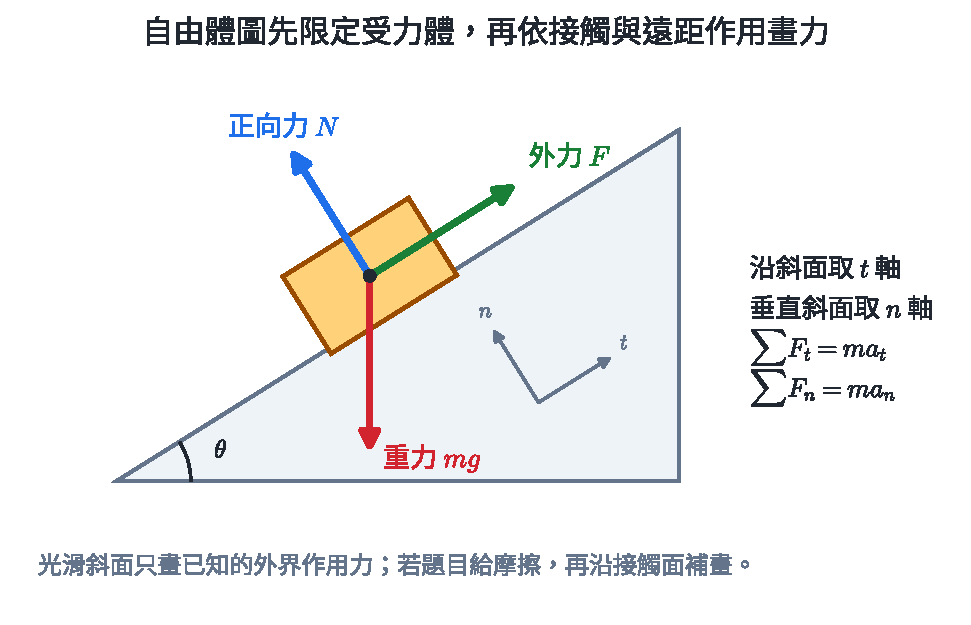
\includegraphics[width=0.96\linewidth,height=\textheight,keepaspectratio,alt={圖 2｜自由體圖先限定受力體；斜面題通常選沿斜面與垂直斜面的座標。}]{assets/選物I-4-受力圖.pdf}
\caption{圖 2｜自由體圖先限定受力體；斜面題通常選沿斜面與垂直斜面的座標。}
\end{figure}

\subsection{\texorpdfstring{\(F\)--\(a\) 與 \(a\)--\(1/M\) 實驗}{F--a 與 a--1/M 實驗}}\label{fa-ux8207-a1m-ux5be6ux9a57}

\begin{figure}
\centering
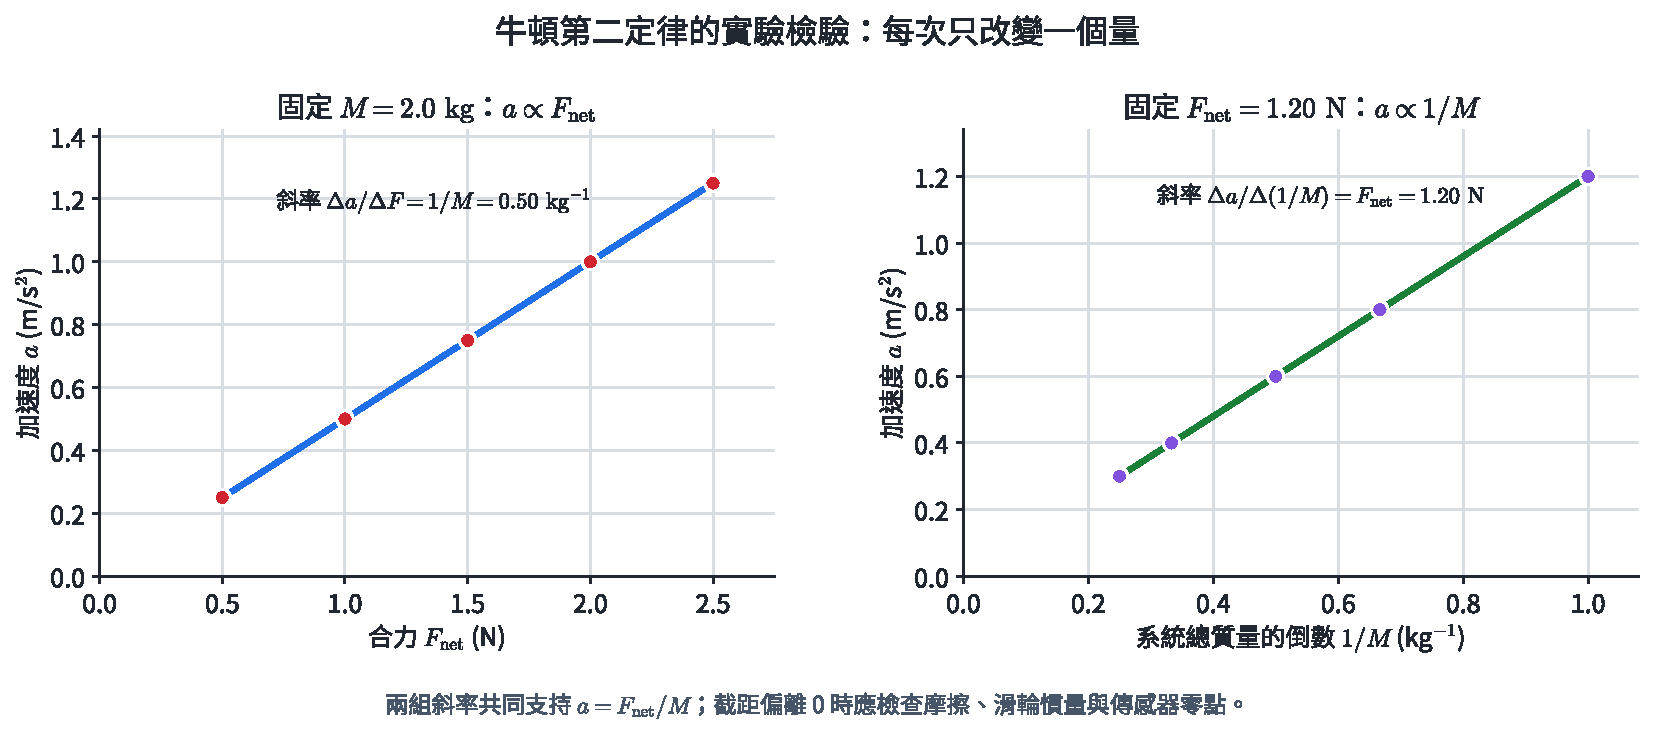
\includegraphics[width=0.98\linewidth,height=\textheight,keepaspectratio,alt={圖 2A｜左圖固定系統總質量 M，測得 a\textbackslash propto F\_\{\textbackslash mathrm\{net\}\}；右圖固定合力，測得 a\textbackslash propto1/M。兩圖的斜率分別對應 1/M 與 F\_\{\textbackslash mathrm\{net\}\}。}]{assets/選物I-4-牛頓第二定律實驗.pdf}
\caption{圖 2A｜左圖固定系統總質量 \(M\)，測得 \(a\propto F_{\mathrm{net}}\)；右圖固定合力，測得 \(a\propto1/M\)。兩圖的斜率分別對應 \(1/M\) 與 \(F_{\mathrm{net}}\)。}
\end{figure}

檢驗力、質量與加速度的關係時，每次只改變一個自變量：

\begin{itemize}
\tightlist
\item
  固定 \(M\)，改變 \(F_{\mathrm{net}}\)，畫 \(a\) 對 \(F_{\mathrm{net}}\)；
\item
  固定 \(F_{\mathrm{net}}\)，改變 \(M\)，把橫軸改為 \(1/M\)，畫 \(a\) 對 \(1/M\)。
\end{itemize}

圖 2A 的兩組直線關係支持下列模型。在慣性參考系中，

\[
\boxed{\sum\vec F=m\vec a}.
\]

在實驗系統中，式中的 \(m\) 是一起加速的完整系統總質量。滑車、附加砝碼與隨繩一起運動的部件都需依實驗邊界納入。最佳直線的截距偏離 0 時，可檢查摩擦、滑輪慣量、桌面水平與感測器零點。

\begin{HandoutWorkedExample}

\subsection{\texorpdfstring{完整示範｜由 \(a\)--\(F_{\mathrm{net}}\) 圖的斜率求系統質量}{完整示範｜由 a--F\_\{\textbackslash mathrm\{net\}\} 圖的斜率求系統質量}}\label{ux5b8cux6574ux793aux7bc4ux7531-af_mathrmnet-ux5716ux7684ux659cux7387ux6c42ux7cfbux7d71ux8ceaux91cf}

固定系統質量，將 \(a\) 畫在縱軸、\(F_{\mathrm{net}}\) 畫在橫軸，最佳直線斜率為 \(0.40\ \mathrm{kg^{-1}}\)，截距接近 0。由

\[
a=\frac1mF_{\mathrm{net}}
\]

得

\[
\frac1m=0.40\ \mathrm{kg^{-1}}
\quad\Rightarrow\quad
m=2.5\ \mathrm{kg}.
\]

斜率單位 \((\mathrm{m/s^2})/\mathrm N=1/\mathrm{kg}\) 與 \(1/m\) 一致。

\end{HandoutWorkedExample}

\begin{HandoutWorkedExample}

\subsection{\texorpdfstring{完整示範｜由 \(a\)--\(1/m\) 圖的斜率求合力}{完整示範｜由 a--1/m 圖的斜率求合力}}\label{ux5b8cux6574ux793aux7bc4ux7531-a1m-ux5716ux7684ux659cux7387ux6c42ux5408ux529b}

固定合力，畫出 \(a\) 對 \(1/m\) 的直線，斜率為 \(1.60\ \mathrm N\)，截距接近 0。因為

\[
a=F_{\mathrm{net}}\left(\frac1m\right),
\]

斜率就是 \(F_{\mathrm{net}}=1.60\ \mathrm N\)。當 \(m=2.00\ \mathrm{kg}\)，

\[
a=\frac{1.60}{2.00}=0.800\ \mathrm{m/s^2}.
\]

改畫 \(1/m\) 將反比關係線性化，可以直接由斜率回推合力。

\end{HandoutWorkedExample}

\begin{HandoutSelfCheck}

\subsection{練習｜第二定律的圖線證據}\label{ux7df4ux7fd2ux7b2cux4e8cux5b9aux5f8bux7684ux5716ux7ddaux8b49ux64da}

\begin{enumerate}
\def\labelenumi{\arabic{enumi}.}
\tightlist
\item
  質量 \(2.0\ \mathrm{kg}\) 物體受 \(6.0\ \mathrm N\) 向右與 \(2.0\ \mathrm N\) 向左，求加速度。
\item
  \(a\) 對 \(F_{\mathrm{net}}\) 圖斜率為 \(0.25\ \mathrm{kg^{-1}}\)，求系統質量。
\item
  \(a\) 對 \(1/m\) 圖斜率為 \(2.4\ \mathrm N\)，求合力。
\item
  檢驗 \(a\propto F_{\mathrm{net}}\) 時，每次增加驅動力卻也同時把砝碼加在滑車上。指出需固定的量。
\item
  某最佳線為 \(a=0.50F_{\mathrm{net}}-0.12\)（SI 單位）。求斜率對應的質量，並提出一個截距偏離 0 的可檢查因素。
\end{enumerate}

\textbf{簡答：}1. \(2.0\ \mathrm{m/s^2}\) 向右。2. \(4.0\ \mathrm{kg}\)。3. \(2.4\ \mathrm N\)。4. 系統總質量 \(m\)。5. \(m=2.0\ \mathrm{kg}\)；可檢查摩擦、零點或桌面傾斜。

\end{HandoutSelfCheck}

分量形式：

\[
\sum F_x=ma_x,
\qquad
\sum F_y=ma_y.
\]

\(\sum\vec F\) 表示同一受力體上所有外力的向量和。計算流程如下：

\begin{enumerate}
\def\labelenumi{\arabic{enumi}.}
\tightlist
\item
  隔離受力體。
\item
  從周遭施力者逐一找力；只畫真實交互作用。
\item
  選讓加速度或接觸面簡單的座標軸。
\item
  把力分解後，逐軸列 \(\sum F=ma\)。
\item
  用方向、單位與極端情形檢查答案。
\end{enumerate}

\subsection{常見力與必要條件}\label{ux5e38ux898bux529bux8207ux5fc5ux8981ux689dux4ef6}

{\def\LTcaptype{none} % do not increment counter
\begin{longtable}[]{@{}
  >{\raggedright\arraybackslash}p{(\linewidth - 4\tabcolsep) * \real{0.3333}}
  >{\raggedright\arraybackslash}p{(\linewidth - 4\tabcolsep) * \real{0.3333}}
  >{\raggedright\arraybackslash}p{(\linewidth - 4\tabcolsep) * \real{0.3333}}@{}}
\toprule\noalign{}
\begin{minipage}[b]{\linewidth}\raggedright
力
\end{minipage} & \begin{minipage}[b]{\linewidth}\raggedright
方向／大小如何決定
\end{minipage} & \begin{minipage}[b]{\linewidth}\raggedright
列式時保留的條件
\end{minipage} \\
\midrule\noalign{}
\endhead
\bottomrule\noalign{}
\endlastfoot
重力 & 近地表 \(\vec W=m\vec g\)，向下 & 質量以 kg 表示；重量是以 N 表示的力 \\
正向力 \(N\) & 垂直接觸面，由限制條件與方程求 & 水平靜止且無額外垂直力時才有 \(N=mg\) \\
張力 \(T\) & 沿繩、拉離受力體；理想輕繩配合理想滑輪時同繩量值相同 & 由各受力體的加速度方程求量值；平衡懸掛時才等於重量 \\
彈簧力 & 比例限度內 \(\vec F_s=-k\vec x\) & 方向由形變決定，運動方向另由速度判斷 \\
摩擦作用 & 平行接觸面、阻礙接觸面間相對滑動趨勢 & 本冊本章不以摩擦係數公式為計算主線 \\
\end{longtable}
}

\subsection{跨冊／大考整合：摩擦係數只留判讀骨架}\label{ux8de8ux518aux5927ux8003ux6574ux5408ux6469ux64e6ux4fc2ux6578ux53eaux7559ux5224ux8b80ux9aa8ux67b6}

{C3 跨冊整合｜摩擦係數計算屬後續章節}

若題目另給摩擦係數模型，先判斷接觸面是否已相對滑動：

\[
0\le f_s\le \mu_sN,
\qquad
f_k=\mu_kN.
\]

靜摩擦力 \(f_s\) 會在上限內調整，剛好阻止相對滑動；\(\mu_sN\) 是最大值，不是每次都取到。已滑動時才使用動摩擦近似 \(f_k=\mu_kN\)。兩者方向都反抗接觸面間的\textbf{相對滑動或滑動趨勢}，不一定與物體速度相反。

\begin{HandoutSelfCheck}

\subsection{練習｜靜摩擦力的調整範圍}\label{ux7df4ux7fd2ux975cux6469ux64e6ux529bux7684ux8abfux6574ux7bc4ux570d}

水平推力 \(2\ \mathrm N\) 作用在仍靜止的箱子上，已知最大靜摩擦力為 \(5\ \mathrm N\)。靜摩擦力量值是多少？

\textbf{答案：}\(2\ \mathrm N\)，方向與推力相反。箱子仍靜止表示水平合力為 0；\(5\ \mathrm N\) 只是靜摩擦可達的上限。

\end{HandoutSelfCheck}

\subsection{斜面與正向力}\label{ux659cux9762ux8207ux6b63ux5411ux529b}

光滑斜面傾角 \(\theta\)，若物體沒有離開或穿入斜面，垂直斜面加速度為 0。只有重力的垂直分量時：

\begin{figure}
\centering
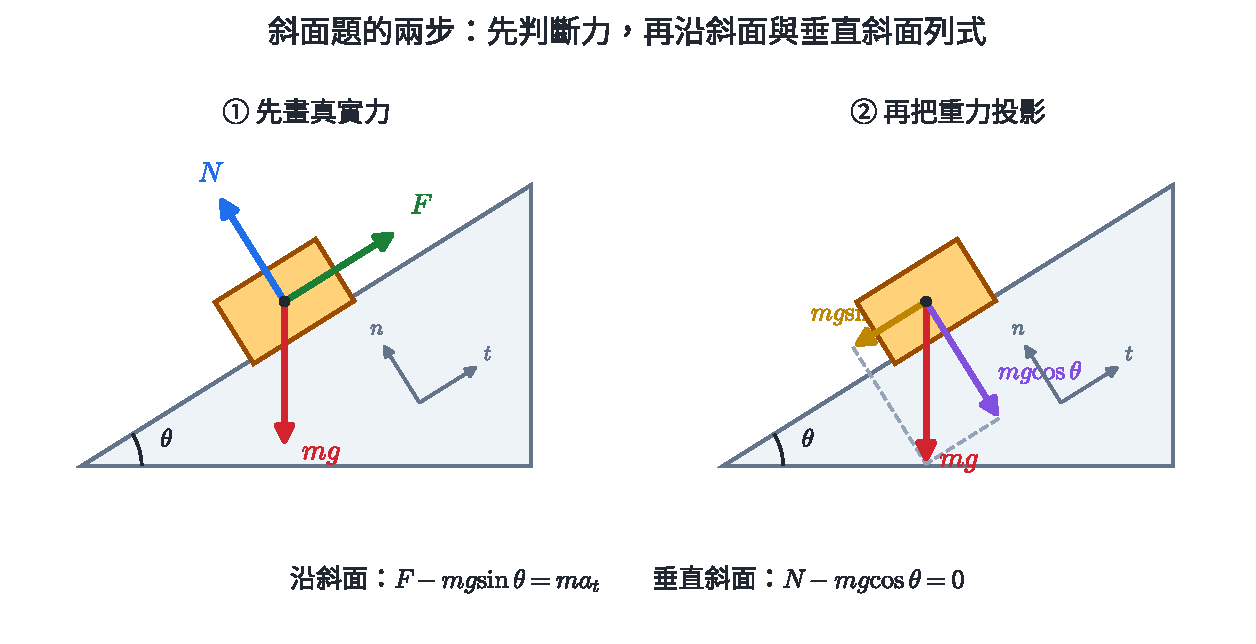
\includegraphics[width=0.96\linewidth,height=\textheight,keepaspectratio,alt={圖 3｜左圖先保留 N、mg 與沿斜面外力；右圖才把 mg 投影為沿斜面的 mg\textbackslash sin\textbackslash theta 與垂直斜面的 mg\textbackslash cos\textbackslash theta。}]{assets/選物I-4-斜面重力分解.pdf}
\caption{圖 3｜左圖先保留 \(N\)、\(mg\) 與沿斜面外力；右圖才把 \(mg\) 投影為沿斜面的 \(mg\sin\theta\) 與垂直斜面的 \(mg\cos\theta\)。}
\end{figure}

圖 3 的 \(t\) 軸沿斜面、\(n\) 軸垂直斜面。沿 \(t\) 軸的重力分量使物體下滑；沿 \(n\) 軸的分量由正向力平衡，因此兩個分量要分別進入兩條方程。

\[
N-mg\cos\theta=0
\quad\Rightarrow\quad
N=mg\cos\theta.
\]

這個結果適用於上述受力條件；斜向拉力、斜面本身加速或失去接觸都會改變 \(N\)。

\begin{HandoutWorkedExample}

\subsection{完整示範｜光滑斜面上的外加力}\label{ux5b8cux6574ux793aux7bc4ux5149ux6ed1ux659cux9762ux4e0aux7684ux5916ux52a0ux529b}

\(m=2.0\ \mathrm{kg}\) 的物體在 \(37^\circ\) 光滑斜面，受沿斜面向上 \(20\ \mathrm N\) 的力，取 \(g=10\ \mathrm{m/s^2}\)、\(\sin37^\circ=0.6\)、\(\cos37^\circ=0.8\)。

沿斜面向上為正：

\[
20-mg\sin37^\circ=ma
\]

\[
20-(2.0)(10)(0.6)=(2.0)a
\Rightarrow a=4.0\ \mathrm{m/s^2}.
\]

垂直斜面方向 \(N=mg\cos37^\circ=16\ \mathrm N\)。

\end{HandoutWorkedExample}

\begin{HandoutWorkedExample}

\subsection{完整示範｜由指定加速度反求繩張力}\label{ux5b8cux6574ux793aux7bc4ux7531ux6307ux5b9aux52a0ux901fux5ea6ux53cdux6c42ux7e69ux5f35ux529b}

\(3.0\ \mathrm{kg}\) 物體在 \(30^\circ\) 光滑斜面上，繩張力沿斜面向上，使物體向上加速度為 \(2.0\ \mathrm{m/s^2}\)。取 \(g=10\ \mathrm{m/s^2}\)。

依圖 3 畫 \(T\)、\(N\)、\(mg\)，沿斜面向上為正：

\[
T-mg\sin30^\circ=ma.
\]

\[
T=(3.0)\left[10(0.5)+2.0\right]=21\ \mathrm N.
\]

垂直斜面方向：

\[
N=mg\cos30^\circ=15\sqrt3\ \mathrm N.
\]

本題由加速度條件反推合力；物體當下速度的方向不進入此力學方程。

\end{HandoutWorkedExample}

\begin{HandoutSelfCheck}

\subsection{練習｜斜面模型}\label{ux7df4ux7fd2ux659cux9762ux6a21ux578b}

\begin{enumerate}
\def\labelenumi{\arabic{enumi}.}
\tightlist
\item
  \(4.0\ \mathrm{kg}\) 物體在 \(30^\circ\) 光滑斜面上自由下滑，求 \(a\) 與 \(N\)。取 \(g=10\ \mathrm{m/s^2}\)。
\item
  上題若另施加沿斜面向上 \(28\ \mathrm N\) 的力，求加速度。
\item
  \(5.0\ \mathrm{kg}\) 物體在 \(37^\circ\) 斜面上保持靜止，沒有其他沿斜面外力。求靜摩擦力的量值與方向。取 \(g=10\ \mathrm{m/s^2}\)、\(\sin37^\circ=0.6\)。
\item
  物塊在斜面上受一支斜向離開斜面的拉力。說明正向力相較於沒有拉力時如何改變。
\end{enumerate}

\textbf{簡答：}1. \(a=5.0\ \mathrm{m/s^2}\) 向下，\(N=20\sqrt3\ \mathrm N\)。2. \(a=2.0\ \mathrm{m/s^2}\) 向上。3. \(30\ \mathrm N\) 沿斜面向上。4. 拉力的離面分量分擔垂直方向的平衡，\(N\) 減小。

\end{HandoutSelfCheck}

\subsection{視重：秤量到的是接觸力}\label{ux8996ux91cdux79e4ux91cfux5230ux7684ux662fux63a5ux89f8ux529b}

\begin{figure}
\centering
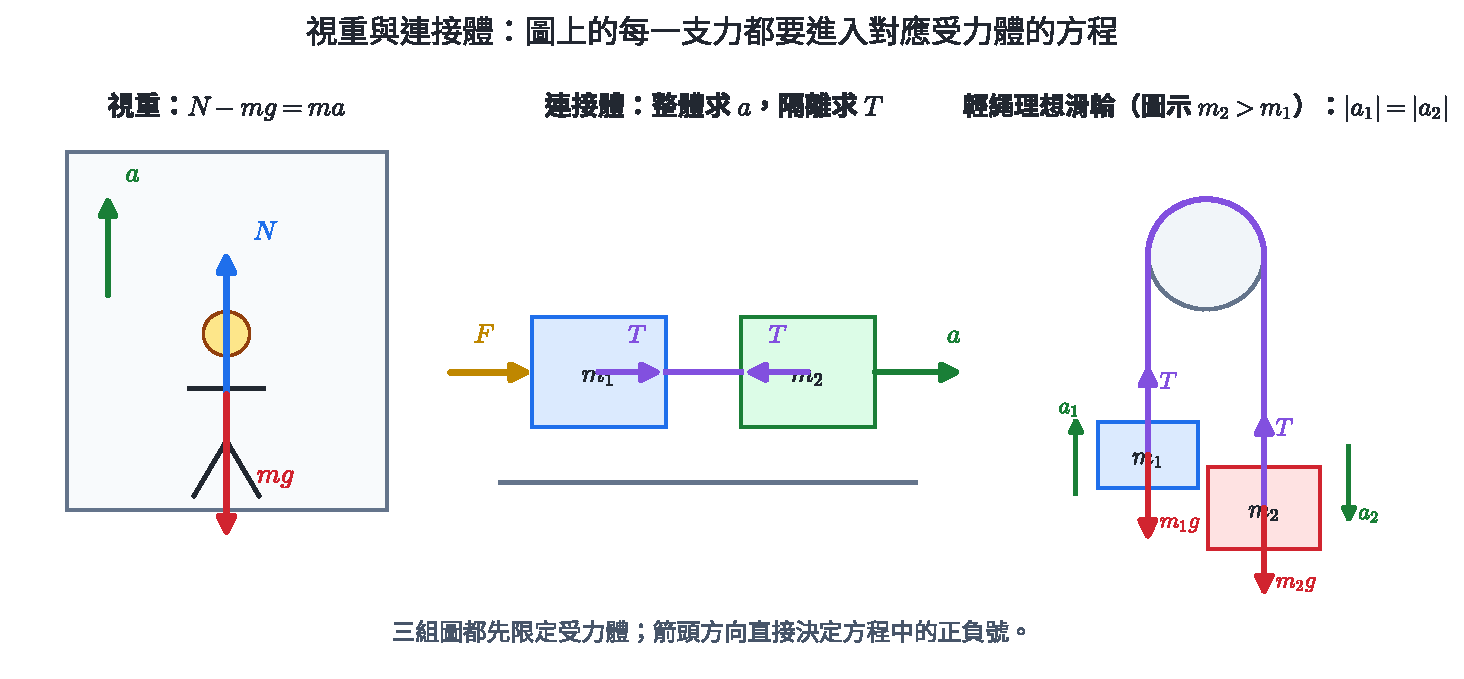
\includegraphics[width=0.98\linewidth,height=\textheight,keepaspectratio,alt={圖 3A｜左圖是電梯中人的自由體圖；中圖在兩塊上分別標出張力；右圖的繩沿滑輪彎形貼合，並以 m\_2\textgreater m\_1 為例標出等量反向的加速度。}]{assets/選物I-4-視重與連接體.pdf}
\caption{圖 3A｜左圖是電梯中人的自由體圖；中圖在兩塊上分別標出張力；右圖的繩沿滑輪彎形貼合，並以 \(m_2>m_1\) 為例標出等量反向的加速度。}
\end{figure}

人在電梯內站上秤，秤的讀數對應正向力量值 \(N\)。取向上為正：

\[
N-mg=ma
\quad\Rightarrow\quad
\boxed{N=m(g+a)}.
\]

向上加速時 \(N>mg\)；向下加速時 \(N<mg\)。速度向上或向下本身不決定讀數，\textbf{加速度方向}才決定。

\subsection{秤讀數是支持力，會隨加速度改變}\label{ux79e4ux8b80ux6578ux662fux652fux6301ux529bux6703ux96a8ux52a0ux901fux5ea6ux6539ux8b8a}

秤感測支撐力 \(N\)。電梯加速時，同一個人的 \(N\) 會改變，因此控制系統估載重時須知道動態狀態，或在穩定條件下校正。自由落下時，人與秤同時以 \(g\) 向下加速，秤無須提供支撐力，讀數為 0；人的質量仍維持不變。

\begin{HandoutWorkedExample}

\subsection{完整示範｜向上運動但速率減少的電梯}\label{ux5b8cux6574ux793aux7bc4ux5411ux4e0aux904bux52d5ux4f46ux901fux7387ux6e1bux5c11ux7684ux96fbux68af}

\(60\ \mathrm{kg}\) 乘客站在秤上。電梯向上運動，以 \(2.0\ \mathrm{m/s^2}\) 的加速度量值減速，取 \(g=10\ \mathrm{m/s^2}\)。

依圖 3A 左圖，向上為正。向上運動且減速，所以 \(a=-2.0\ \mathrm{m/s^2}\)：

\[
N=m(g+a)=60(10-2)=480\ \mathrm N.
\]

讀值小於靜止時的 \(mg=600\ \mathrm N\)。

\end{HandoutWorkedExample}

\begin{HandoutWorkedExample}

\subsection{完整示範｜由秤讀值判斷加速度}\label{ux5b8cux6574ux793aux7bc4ux7531ux79e4ux8b80ux503cux5224ux65b7ux52a0ux901fux5ea6}

\(60\ \mathrm{kg}\) 乘客的秤讀值對應 \(N=720\ \mathrm N\)，取 \(g=10\ \mathrm{m/s^2}\)。

\[
720-600=60a
\quad\Rightarrow\quad
a=+2.0\ \mathrm{m/s^2}.
\]

加速度向上。電梯若當下向下運動，速率正在減少；若向上運動，速率正在增加。

\end{HandoutWorkedExample}

\begin{HandoutSelfCheck}

\subsection{練習｜電梯視重}\label{ux7df4ux7fd2ux96fbux68afux8996ux91cd}

\begin{enumerate}
\def\labelenumi{\arabic{enumi}.}
\tightlist
\item
  \(50\ \mathrm{kg}\) 人在靜止電梯內，取 \(g=10\ \mathrm{m/s^2}\)，求 \(N\)。
\item
  上題電梯以 \(3.0\ \mathrm{m/s^2}\) 向上加速，求 \(N\)。
\item
  上題電梯以 \(3.0\ \mathrm{m/s^2}\) 向下加速，求 \(N\)。
\item
  電梯與乘客同時自由落下的理想極限中，求 \(N\)，並說明乘客質量是否改變。
\end{enumerate}

\textbf{簡答：}1. \(500\ \mathrm N\)。2. \(650\ \mathrm N\)。3. \(350\ \mathrm N\)。4. \(N=0\)；質量不變。

\end{HandoutSelfCheck}

\subsection{連接體：整體求加速度，隔離求內力}\label{ux9023ux63a5ux9ad4ux6574ux9ad4ux6c42ux52a0ux901fux5ea6ux9694ux96e2ux6c42ux5167ux529b}

理想輕繩不可伸長，連接物沿繩方向具有相同加速度量值。把整個系統視為一體時，張力等內力互相抵銷，可先求共同 \(a\)；要找張力或接觸力，必須再隔離其中一物體。

\begin{HandoutWorkedExample}

\subsection{完整示範｜水平面上兩物塊的接觸力}\label{ux5b8cux6574ux793aux7bc4ux6c34ux5e73ux9762ux4e0aux5169ux7269ux584aux7684ux63a5ux89f8ux529b}

圖 3A 中圖的光滑水平面上，\(m_1=2.0\ \mathrm{kg}\)、\(m_2=3.0\ \mathrm{kg}\)，以 \(20\ \mathrm N\) 向右推左側物塊。先把兩塊視為整體：

\[
a=\frac{F}{m_1+m_2}
=\frac{20}{5.0}
=4.0\ \mathrm{m/s^2}.
\]

再隔離 \(m_2\)，它的水平合力只有 \(m_1\) 對它的接觸力 \(C\)：

\[
C=m_2a=(3.0)(4.0)=12\ \mathrm N.
\]

第三定律給出 \(m_2\) 對 \(m_1\) 的接觸力也是 \(12\ \mathrm N\)，方向向左。

\end{HandoutWorkedExample}

\begin{HandoutWorkedExample}

\subsection{完整示範｜阿特伍德機}\label{ux5b8cux6574ux793aux7bc4ux963fux7279ux4f0dux5fb7ux6a5f}

理想滑輪兩側懸掛 \(m_1=1.0\ \mathrm{kg}\)、\(m_2=4.0\ \mathrm{kg}\)，取 \(g=10\ \mathrm{m/s^2}\)。較重的 \(m_2\) 向下：

\[
m_2g-T=m_2a,
\qquad
T-m_1g=m_1a.
\]

相加消去 \(T\)：

\[
a=\frac{m_2-m_1}{m_1+m_2}g=6.0\ \mathrm{m/s^2}.
\]

代回 \(T-m_1g=m_1a\)，得 \(T=16\ \mathrm N\)。

\end{HandoutWorkedExample}

\begin{HandoutSelfCheck}

\subsection{練習｜連接體}\label{ux7df4ux7fd2ux9023ux63a5ux9ad4}

\begin{enumerate}
\def\labelenumi{\arabic{enumi}.}
\tightlist
\item
  光滑水平面上 \(1.0\ \mathrm{kg}\) 與 \(3.0\ \mathrm{kg}\) 物塊以輕繩相連，\(12\ \mathrm N\) 向右拉右塊。求 \(a\)、\(T\)。
\item
  上題改為 \(12\ \mathrm N\) 向左拉左塊，求 \(a\)、\(T\) 的量值。
\item
  阿特伍德機 \(m_1=2.0\ \mathrm{kg}\)、\(m_2=3.0\ \mathrm{kg}\)，取 \(g=10\ \mathrm{m/s^2}\)，求 \(a\)、\(T\)。
\item
  阿特伍德機兩側質量同時加倍，比較 \(a\) 與 \(T\)。
\item
  繩的質量不可忽略時，說明為何張力可能沿繩改變。
\end{enumerate}

\textbf{簡答：}1. \(a=3.0\ \mathrm{m/s^2}\) 向右、\(T=3.0\ \mathrm N\)。2. \(a=3.0\ \mathrm{m/s^2}\) 向左、\(T=9.0\ \mathrm N\)。3. \(a=2.0\ \mathrm{m/s^2}\)、\(T=24\ \mathrm N\)。4. \(a\) 不變，\(T\) 加倍。5. 繩段本身需要合力來加速，其兩端張力有差。

\end{HandoutSelfCheck}

\begin{HandoutSelfCheck}

\subsection{練習}\label{ux7df4ux7fd2-3}

一物體在水平面上，受到向右 \(9\ \mathrm N\) 與向左 \(3\ \mathrm N\)，質量 \(2\ \mathrm{kg}\)。加速度為何？

\textbf{答案：}合力向右 \(6\ \mathrm N\)，所以 \(a=6/2=3\ \mathrm{m/s^2}\) 向右。不能把其中 \(9\ \mathrm N\) 單獨設成 \(ma\)。

\end{HandoutSelfCheck}

\section{4. 牛頓第三定律：每個交互作用都有兩端}\label{ux725bux9813ux7b2cux4e09ux5b9aux5f8bux6bcfux500bux4ea4ux4e92ux4f5cux7528ux90fdux6709ux5169ux7aef}

\begin{figure}
\centering
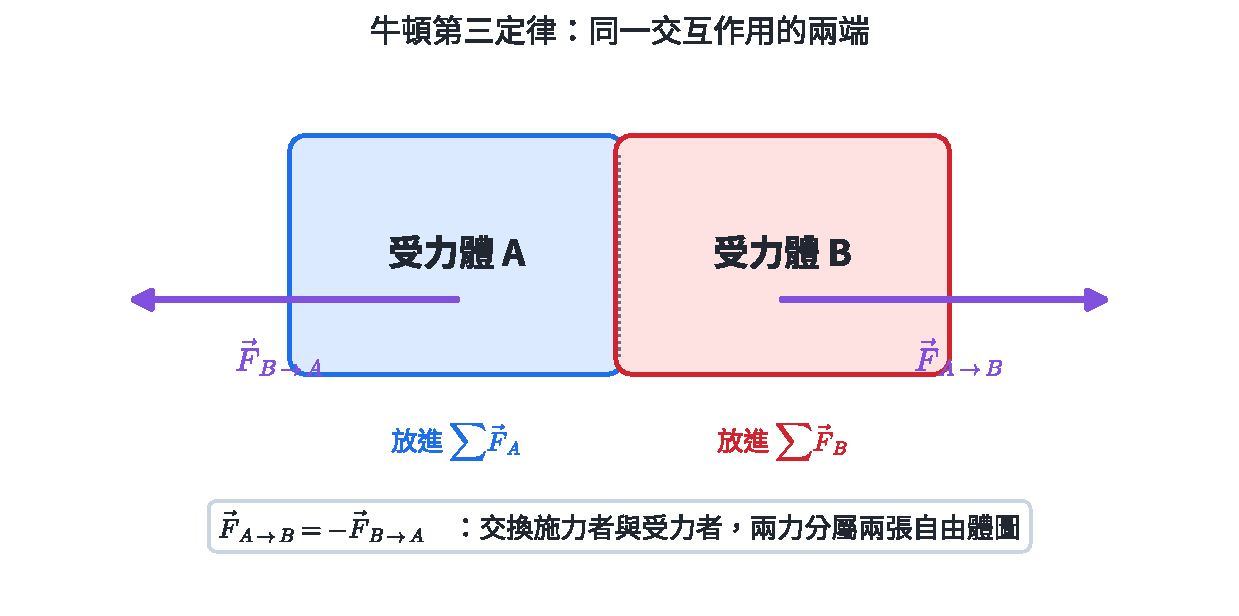
\includegraphics[width=0.96\linewidth,height=\textheight,keepaspectratio,alt={圖 4｜紫色兩箭頭是同一交互作用的兩端：\textbackslash vec F\_\{B\textbackslash to A\} 只放進 A 的自由體圖，\textbackslash vec F\_\{A\textbackslash to B\} 只放進 B 的自由體圖。}]{assets/選物I-4-第三定律力對.pdf}
\caption{圖 4｜紫色兩箭頭是同一交互作用的兩端：\(\vec F_{B\to A}\) 只放進 A 的自由體圖，\(\vec F_{A\to B}\) 只放進 B 的自由體圖。}
\end{figure}

A 作用在 B 的力與 B 作用在 A 的力：

\[
\boxed{\vec F_{A\to B}=-\vec F_{B\to A}}.
\]

它們量值相等、方向相反、同時出現、屬於同一種交互作用，但\textbf{作用在不同物體上}。因此不會在某一物體的 \(\sum\vec F\) 中互相抵銷。

圖 4 的下標先寫施力者、箭頭後寫受力者。交換兩者便得到配對力；受力者不同，所以列某一物體的 \(\sum\vec F\) 時只會收進其中一支。

{\def\LTcaptype{none} % do not increment counter
\begin{longtable}[]{@{}lll@{}}
\toprule\noalign{}
判斷 & 第三定律力對 & 同一物體上的兩個力 \\
\midrule\noalign{}
\endhead
\bottomrule\noalign{}
\endlastfoot
作用在哪裡 & 不同物體 & 同一物體 \\
力的種類 & 同一交互作用兩端 & 可以是不同交互作用 \\
是否必等大反向 & 是 & 兩者是僅有的兩力且合力為 0 時才等大反向 \\
\end{longtable}
}

例如書靜止在水平桌面上且只受重力與正向力：兩力作用在同一本書上，等大反向並使合力為 0，但不是第三定律力對。重力的配對是書拉地球；正向力的配對是書壓桌面。

\begin{HandoutWorkedExample}

\subsection{完整示範｜書與桌面中的兩組交互作用}\label{ux5b8cux6574ux793aux7bc4ux66f8ux8207ux684cux9762ux4e2dux7684ux5169ux7d44ux4ea4ux4e92ux4f5cux7528}

書靜止在桌上，以書為受力體：

\[
N-mg=0.
\]

重力與正向力都作用在書上，分別來自地球引力與桌面接觸。它們的配對為：

\begin{itemize}
\tightlist
\item
  地球對書的引力 ↔ 書對地球的引力；
\item
  桌面對書的正向力 ↔ 書對桌面的接觸力。
\end{itemize}

平衡方程說明書的加速度；第三定律說明交互作用如何連接兩個物體。

\end{HandoutWorkedExample}

\begin{HandoutWorkedExample}

\subsection{完整示範｜小車與卡車碰撞的力與加速度}\label{ux5b8cux6574ux793aux7bc4ux5c0fux8ecaux8207ux5361ux8ecaux78b0ux649eux7684ux529bux8207ux52a0ux901fux5ea6}

碰撞某一瞬間，卡車對 \(1000\ \mathrm{kg}\) 小車的力為 \(6000\ \mathrm N\) 向左。小車對 \(2000\ \mathrm{kg}\) 卡車的力為 \(6000\ \mathrm N\) 向右。若碰撞力主導各自水平合力：

\[
|a_{\mathrm{car}}|=\frac{6000}{1000}=6.0\ \mathrm{m/s^2},
\]

\[
|a_{\mathrm{truck}}|=\frac{6000}{2000}=3.0\ \mathrm{m/s^2}.
\]

交互作用力等大，質量較小的小車具有較大加速度量值。

\end{HandoutWorkedExample}

\subsection{火箭以排出質量獲得反作用力}\label{ux706bux7badux4ee5ux6392ux51faux8ceaux91cfux7372ux5f97ux53cdux4f5cux7528ux529b}

火箭把燃氣向後加速，同時受到燃氣向前的作用力。第三定律的交互作用發生在火箭與噴出的燃氣之間，因此真空中仍能產生推力。兩力分別作用在燃氣與火箭；分析火箭時只收集燃氣對火箭的力。

\begin{HandoutSelfCheck}

\subsection{練習}\label{ux7df4ux7fd2-4}

小車撞大卡車時，哪一方受到的碰撞力量值較大？哪一方加速度通常較大？

\textbf{答案：}相互作用力量值相等、方向相反；小車質量較小，同樣力下加速度量值通常較大。力相等不代表運動改變相等。

\end{HandoutSelfCheck}

\begin{HandoutSelfCheck}

\subsection{練習｜第三定律力對}\label{ux7df4ux7fd2ux7b2cux4e09ux5b9aux5f8bux529bux5c0d}

\begin{enumerate}
\def\labelenumi{\arabic{enumi}.}
\tightlist
\item
  人向下壓秤，寫出秤對人之力的配對力。
\item
  地球拉蘋果與蘋果拉地球的力量值如何比較？加速度量值如何比較？
\item
  人用 \(80\ \mathrm N\) 向右推牽引車，牽引車對人的力為何？
\item
  說明力對為何分屬兩個合力式。
\item
  溜冰的甲、乙互推，乙質量是甲的 2 倍。比較推力與加速度量值。
\end{enumerate}

\textbf{簡答：}1. 人對秤向下的力。2. 力等大反向；蘋果加速度量值遠大於地球。3. \(80\ \mathrm N\) 向左。4. 兩力的受力者不同。5. 推力等大；甲的加速度量值是乙的 2 倍。

\end{HandoutSelfCheck}

\section{Part B｜從速度轉向到週期振盪}\label{part-bux5f9eux901fux5ea6ux8f49ux5411ux5230ux9031ux671fux632fux76ea}

\section{5. 等速圓周運動：徑向合力提供向心加速度}\label{ux7b49ux901fux5713ux5468ux904bux52d5ux5f91ux5411ux5408ux529bux63d0ux4f9bux5411ux5fc3ux52a0ux901fux5ea6}

\begin{figure}
\centering
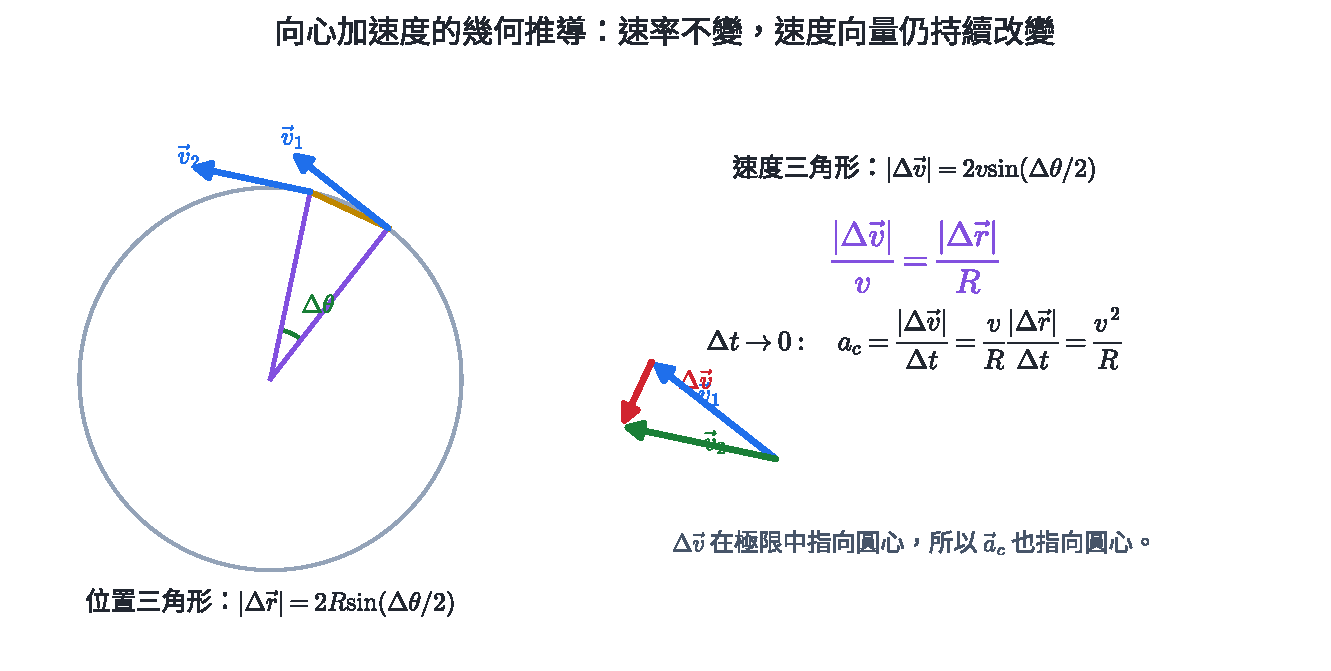
\includegraphics[width=0.98\linewidth,height=\textheight,keepaspectratio,alt={圖 5A｜位置三角形與速度三角形具有相同夾角；當 \textbackslash Delta t 趨近 0，\textbackslash Delta\textbackslash vec v 指向圓心，並得 a\_c=v\^{}2/R。}]{assets/選物I-4-向心加速度推導.pdf}
\caption{圖 5A｜位置三角形與速度三角形具有相同夾角；當 \(\Delta t\) 趨近 0，\(\Delta\vec v\) 指向圓心，並得 \(a_c=v^2/R\)。}
\end{figure}

在固定轉軸下先選定正轉向，例如從紙面外看取逆時針為正。角位置 \(\theta\) 以弧度表示；從 \(\theta_1\) 轉到 \(\theta_2\) 的角位移為

\[
\Delta\theta=\theta_2-\theta_1=\frac{s}{R}.
\]

\(s\) 是帶正負號的弧長：沿正轉向為正，反向為負。弧度是弧長與半徑的比，量綱為 1；書寫角速度時仍保留 rad 以辨識角量。平均角速度與瞬時角速度分別為

\[
\bar\omega=\frac{\Delta\theta}{\Delta t},
\qquad
\omega=\lim_{\Delta t\to0}\frac{\Delta\theta}{\Delta t},
\]

單位為 \(\mathrm{rad/s}\)，正負號表示轉動方向。等速圓周運動的角速率是 \(|\omega|\)。

短時間 \(\Delta t\) 內，位置向量轉過 \(\Delta\theta\)，速度向量也轉過同一夾角。圖 5A 的兩個等腰三角形給出

\[
|\Delta\vec r|=2R\sin\frac{\Delta\theta}{2},
\qquad
|\Delta\vec v|=2v\sin\frac{\Delta\theta}{2}.
\]

因此

\[
\frac{|\Delta\vec v|}{v}
=\frac{|\Delta\vec r|}{R}.
\]

當 \(\Delta t\to0\)，\(|\Delta\vec r|/\Delta t\to v\)，故

\[
a_c=\lim_{\Delta t\to0}\frac{|\Delta\vec v|}{\Delta t}
=\frac vR\lim_{\Delta t\to0}\frac{|\Delta\vec r|}{\Delta t}
=\boxed{\frac{v^2}{R}}.
\]

速度差在極限中指向圓心，因此向心加速度與瞬時速度垂直。

每轉一圈的角位移量值為 \(2\pi\) rad，頻率 \(f\) 是每秒圈數，週期 \(T\) 是每圈所需時間。本章在週期公式中以非負的角速率 \(\omega_{\mathrm{speed}}=|\omega|\) 表示轉動快慢，通常簡寫為 \(\omega\)：

\[
f=\frac1T,
\qquad
\boxed{\omega_{\mathrm{speed}}=2\pi f=\frac{2\pi}{T}},
\qquad
\boxed{v=R|\omega|=R\omega_{\mathrm{speed}}=\frac{2\pi R}{T}}.
\]

雖然速率 \(v\) 不變，速度方向沿切線持續改變，所以有指向圓心的加速度：

\[
\boxed{a_c=\frac{v^2}{R}=R\omega^2=\frac{4\pi^2R}{T^2}}.
\]

依牛頓第二定律，指向圓心的合力分量為

\[
\boxed{\sum F_r=ma_c=m\frac{v^2}{R}}.
\]

「向心力」只是這個徑向合力的角色名稱。繩張力、重力、正向力、摩擦作用或數力合成，都可能提供它；自由體圖不再額外畫一支「向心力」。

\begin{figure}
\centering
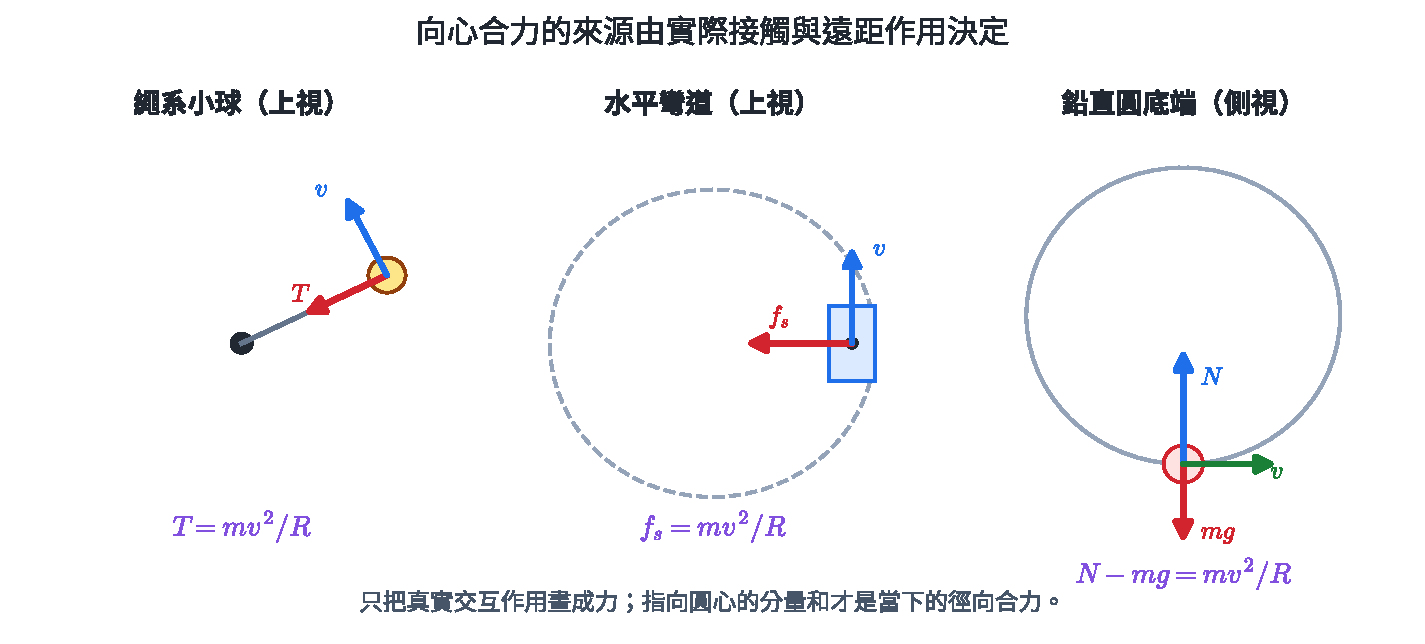
\includegraphics[width=0.98\linewidth,height=\textheight,keepaspectratio,alt={圖 5B｜繩張力、靜摩擦力，或正向力與重力的差，分別在三個模型中提供向心合力。}]{assets/選物I-4-圓周受力模型.pdf}
\caption{圖 5B｜繩張力、靜摩擦力，或正向力與重力的差，分別在三個模型中提供向心合力。}
\end{figure}

圖 5B 的每一個方程都由受力圖沿指向圓心的徑向投影而得。速度箭頭沿切線，只用來確定軌跡與當下轉向方式，不是一支力。

\begin{figure}
\centering
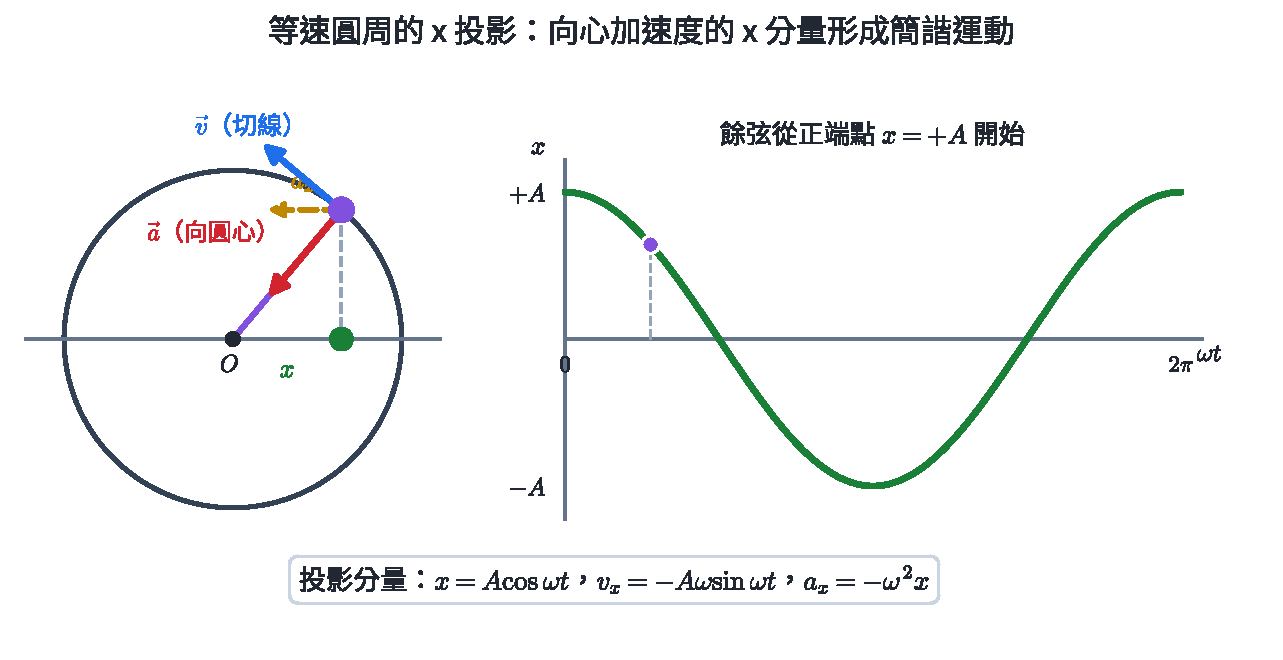
\includegraphics[width=0.96\linewidth,height=\textheight,keepaspectratio,alt={圖 5｜圓周速度沿切線、加速度向圓心；圓周在直徑上的投影會成為簡諧運動。}]{assets/選物I-4-圓周與簡諧.pdf}
\caption{圖 5｜圓周速度沿切線、加速度向圓心；圓周在直徑上的投影會成為簡諧運動。}
\end{figure}

圖 5 的紅箭頭是完整向心加速度 \(\vec a\)；橙色虛線才是它在投影方向的分量 \(a_x=-\omega^2x\)。右側餘弦曲線由 \(t=0\) 的正端點 \(x=+A\) 出發，與本節採用的 \(x=A\cos\omega t\) 相位一致。

\begin{HandoutWorkedExample}

\subsection{完整示範｜旋轉平台上的物體}\label{ux5b8cux6574ux793aux7bc4ux65cbux8f49ux5e73ux53f0ux4e0aux7684ux7269ux9ad4}

\(m=0.50\ \mathrm{kg}\) 的物體以 \(R=0.80\ \mathrm m\)、週期 \(T=2.0\ \mathrm s\) 作等速圓周運動：

\[
v=\frac{2\pi(0.80)}{2.0}=0.80\pi\ \mathrm{m/s},
\]

\[
a_c=\frac{4\pi^2(0.80)}{(2.0)^2}=0.80\pi^2\ \mathrm{m/s^2}.
\]

所需徑向合力量值為 \(ma_c=0.40\pi^2\ \mathrm N\)，方向始終指向圓心。

\end{HandoutWorkedExample}

\begin{HandoutWorkedExample}

\subsection{完整示範｜水平繩系小球}\label{ux5b8cux6574ux793aux7bc4ux6c34ux5e73ux7e69ux7cfbux5c0fux7403}

圖 5B 左圖的 \(0.30\ \mathrm{kg}\) 小球以 \(R=0.60\ \mathrm m\)、\(v=4.0\ \mathrm{m/s}\) 在水平面內繞圈，徑向力只有繩張力。

\[
T=m\frac{v^2}{R}
=(0.30)\frac{4.0^2}{0.60}
=8.0\ \mathrm N.
\]

繩斷的瞬間，小球保留當下切線速度；後續軌跡由斷繩後仍存在的力決定。

\end{HandoutWorkedExample}

\begin{HandoutWorkedExample}

\subsection{完整示範｜水平彎道的最大速率}\label{ux5b8cux6574ux793aux7bc4ux6c34ux5e73ux5f4eux9053ux7684ux6700ux5927ux901fux7387}

\(900\ \mathrm{kg}\) 汽車通過半徑 \(50\ \mathrm m\) 的水平彎道，輪胎與路面可提供的最大水平靜摩擦力為 \(3600\ \mathrm N\)。極限狀態下，圖 5B 中圖的靜摩擦力完全提供向心合力：

\[
3600=900\frac{v_{\max}^2}{50},
\]

\[
v_{\max}=\sqrt{200}\approx14.1\ \mathrm{m/s}.
\]

濕滑路面可提供的最大摩擦力較小，所以安全通過速率也較小。

\end{HandoutWorkedExample}

\begin{HandoutWorkedExample}

\subsection{完整示範｜鉛直圓底端的正向力}\label{ux5b8cux6574ux793aux7bc4ux925bux76f4ux5713ux5e95ux7aefux7684ux6b63ux5411ux529b}

圖 5B 右圖中，\(0.20\ \mathrm{kg}\) 物體通過鉛直圓底端，\(R=0.50\ \mathrm m\)、\(v=4.0\ \mathrm{m/s}\)，取 \(g=9.8\ \mathrm{m/s^2}\)。底端指向圓心的方向向上：

\[
N-mg=m\frac{v^2}{R}.
\]

\[
N=(0.20)(9.8)+(0.20)\frac{16}{0.50}
=8.36\ \mathrm N.
\]

\(N>mg\) 提供了向上合力，使速度向量轉向。

\end{HandoutWorkedExample}

\subsection{向心加速度連結彎道、脫水與離心設備}\label{ux5411ux5fc3ux52a0ux901fux5ea6ux9023ux7d50ux5f4eux9053ux812bux6c34ux8207ux96e2ux5fc3ux8a2dux5099}

速度方向改變得越快，需要的向心加速度越大；\(a_c=v^2/R\) 顯示速率加倍，需求變 4 倍，彎得更急也會增大需求。道路因此以路面作用力的水平分量協助轉彎。滾筒內物體若失去足夠向心作用，就依慣性沿切線離開原圓軌跡；「被甩出」不是多出一種向外基本力，而是約束不足後的運動結果。

\begin{HandoutSelfCheck}

\subsection{練習}\label{ux7df4ux7fd2-5}

同一物體以相同速率繞半徑減半的圓，向心加速度與向心合力變成幾倍？

\textbf{答案：}\(a_c=v^2/R\)，半徑減半使 \(a_c\) 變 2 倍；質量不變，所以所需合力也變 2 倍。

\end{HandoutSelfCheck}

\begin{HandoutSelfCheck}

\subsection{練習｜向心加速度與實際受力}\label{ux7df4ux7fd2ux5411ux5fc3ux52a0ux901fux5ea6ux8207ux5be6ux969bux53d7ux529b}

\begin{enumerate}
\def\labelenumi{\arabic{enumi}.}
\tightlist
\item
  半徑 \(0.50\ \mathrm m\)、頻率 \(2.0\ \mathrm{Hz}\)，求 \(\omega\)、\(v\)、\(a_c\)。
\item
  同一半徑中，週期加倍，\(v\) 與 \(a_c\) 各變為幾倍？
\item
  \(0.40\ \mathrm{kg}\) 小球以 \(R=0.80\ \mathrm m\)、\(v=3.0\ \mathrm{m/s}\) 繞水平圓，徑向力只有張力。求 \(T\)。
\item
  \(1000\ \mathrm{kg}\) 車以 \(10\ \mathrm{m/s}\) 通過 \(R=40\ \mathrm m\) 水平彎道，求所需摩擦力量值。
\item
  鉛直圓底端 \(N=3mg\)，求 \(v^2/R\) 與 \(g\) 的關係。
\item
  彎道半徑不變，可提供的最大徑向力減為原來 \(1/4\)，安全最大速率變為幾倍？
\end{enumerate}

\textbf{簡答：}1. \(4\pi\ \mathrm{rad/s}\)、\(2\pi\ \mathrm{m/s}\)、\(8\pi^2\ \mathrm{m/s^2}\)。2. \(v\) 變 \(1/2\)，\(a_c\) 變 \(1/4\)。3. \(4.5\ \mathrm N\)。4. \(2500\ \mathrm N\) 指向彎道中心。5. \(v^2/R=2g\)。6. \(1/2\)。

\end{HandoutSelfCheck}

\section{6. 簡諧運動：回復力把物體拉回，又因慣性越過平衡點}\label{ux7c21ux8ae7ux904bux52d5ux56deux5fa9ux529bux628aux7269ux9ad4ux62c9ux56deux53c8ux56e0ux6163ux6027ux8d8aux904eux5e73ux8861ux9ede}

\begin{figure}
\centering
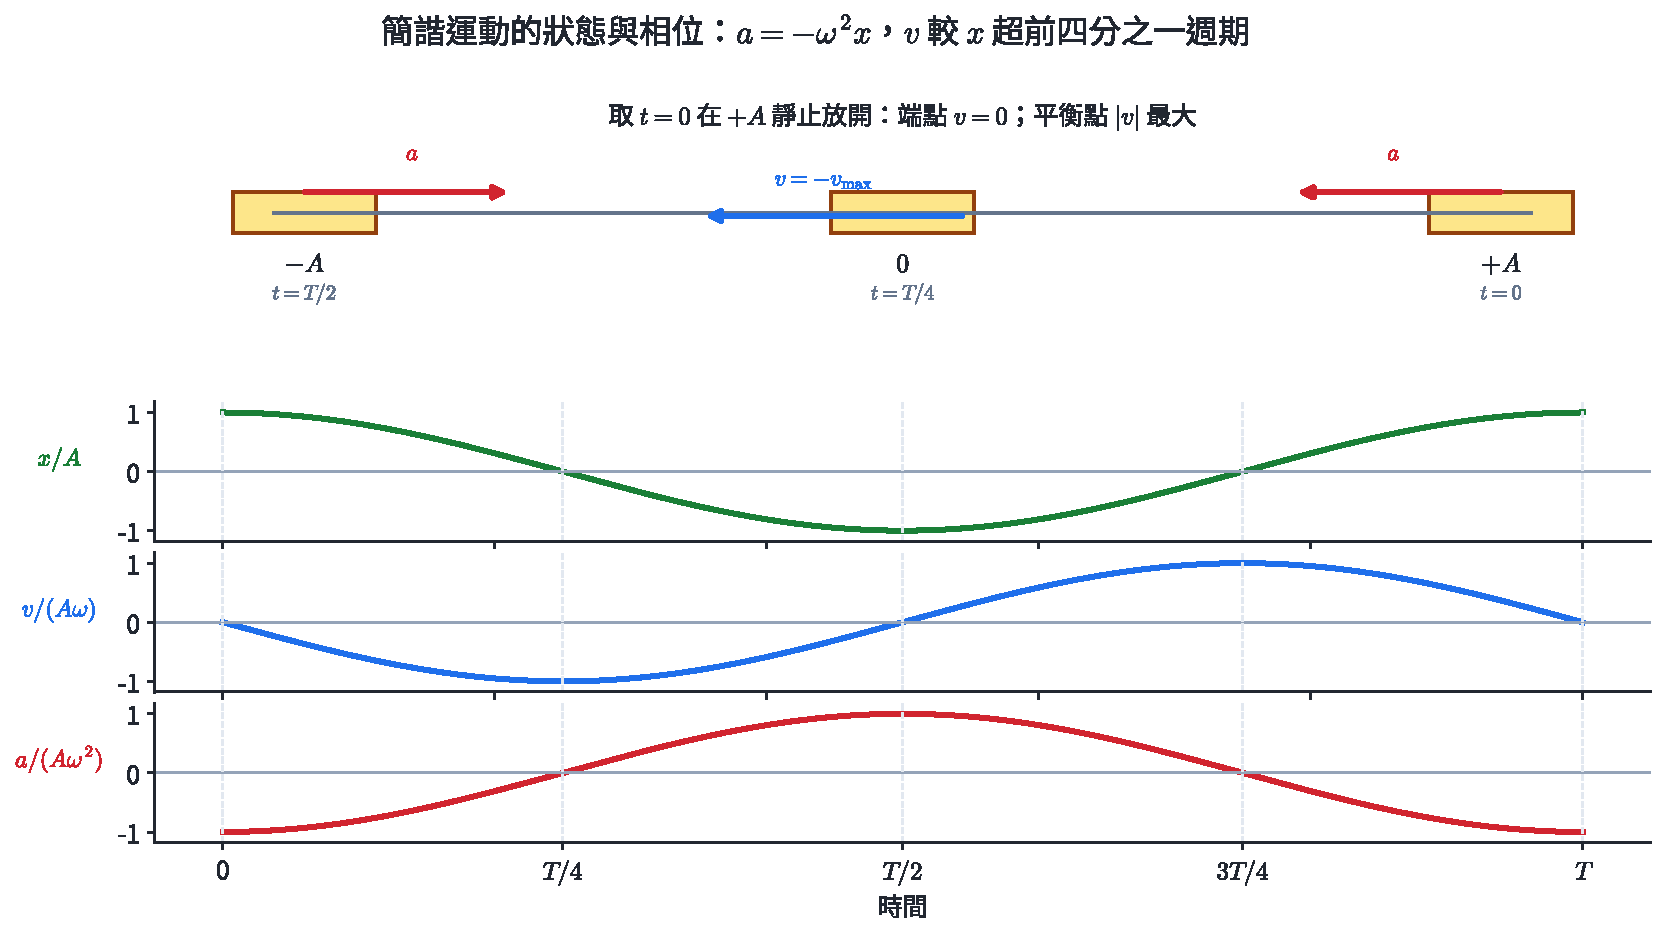
\includegraphics[width=0.98\linewidth,height=\textheight,keepaspectratio,alt={圖 6A｜取 t=0 在 +A 靜止放開：第一次通過平衡點時 v=-v\_\{\textbackslash max\}，到 -A 時速度再為 0。下圖以同一初始條件對齊 x、v、a 三條時間曲線。}]{assets/選物I-4-簡諧狀態與相位.pdf}
\caption{圖 6A｜取 \(t=0\) 在 \(+A\) 靜止放開：第一次通過平衡點時 \(v=-v_{\max}\)，到 \(-A\) 時速度再為 0。下圖以同一初始條件對齊 \(x\)、\(v\)、\(a\) 三條時間曲線。}
\end{figure}

圖 6A 先給出狀態關係：端點的速度為 0，回復加速度量值最大；平衡點的加速度為 0，速率最大。接下來用線性回復力導出這些關係。

理想水平彈簧連接質量 \(m\)，以平衡位置為 \(x=0\)。虎克定律配合牛頓第二定律：

\[
ma=-kx
\quad\Rightarrow\quad
\boxed{a=-\frac{k}{m}x}.
\]

若定義

\[
\omega=\sqrt{\frac{k}{m}},
\]

便有 \(a=-\omega^2x\)。符合「加速度與位移成正比、方向相反」的週期運動叫\textbf{簡諧運動}。若 \(t=0\) 在正端點，可寫

\[
\boxed{x=A\cos\omega t},
\]

\[
\boxed{v=-A\omega\sin\omega t},
\qquad
\boxed{a=-A\omega^2\cos\omega t=-\omega^2x}.
\]

週期與彈簧系統關係：

\[
\boxed{T=\frac{2\pi}{\omega}=2\pi\sqrt{\frac{m}{k}}}.
\]

{\def\LTcaptype{none} % do not increment counter
\begin{longtable}[]{@{}lrr@{}}
\toprule\noalign{}
位置 & 速度量值 & 加速度量值 \\
\midrule\noalign{}
\endhead
\bottomrule\noalign{}
\endlastfoot
端點 \(|x|=A\) & 0 & 最大 \(A\omega^2\) \\
平衡點 \(x=0\) & 最大 \(A\omega\) & 0 \\
\end{longtable}
}

由 \(\sin^2\omega t+\cos^2\omega t=1\) 可消去時間：

\[
\boxed{v^2=\omega^2(A^2-x^2)}.
\]

這條式給出速率量值；速度正負仍由當下運動方向決定。

\subsection{簡諧運動的正弦與餘弦形式}\label{ux7c21ux8ae7ux904bux52d5ux7684ux6b63ux5f26ux8207ux9918ux5f26ux5f62ux5f0f}

半徑 \(A\)、角速率 \(\omega\) 的等速圓周運動，在 \(x\) 軸的投影為 \(x=A\cos\omega t\)；速度與加速度的投影也正好是上式。圓周投影提供幾何模型，不表示做簡諧運動的物體真的繞圓。

\subsection{常見錯誤｜把簡諧運動當等加速度}\label{ux5e38ux898bux932fux8aa4ux628aux7c21ux8ae7ux904bux52d5ux7576ux7b49ux52a0ux901fux5ea6}

\(a=-\omega^2x\) 隨位置改變，不是定值，因此不能把第 2 章的等加速度三式跨整段套用。\(T=2\pi\sqrt{m/k}\) 也依賴理想彈簧、比例限度、阻力可忽略等模型條件。

\subsection{微型加速度計以彈簧形變估計加速度}\label{ux5faeux578bux52a0ux901fux5ea6ux8a08ux4ee5ux5f48ux7c27ux5f62ux8b8aux4f30ux8a08ux52a0ux901fux5ea6}

微機電加速度計內有可微小位移的質量與彈性結構。外殼加速時，內部質量因慣性相對外殼偏移；電路量到位移，再利用已校準的力---位移與動態模型反推加速度。外界變化接近感測結構的固有頻率時，輸出會被放大並產生相位差，因此工程設計須限定工作頻帶，並加入阻尼與校正。

\begin{HandoutWorkedExample}

\subsection{\texorpdfstring{完整示範｜由 \(x(t)\) 讀出整個簡諧運動}{完整示範｜由 x(t) 讀出整個簡諧運動}}\label{ux5b8cux6574ux793aux7bc4ux7531-xt-ux8b80ux51faux6574ux500bux7c21ux8ae7ux904bux52d5}

\[
x=(0.080\ \mathrm m)\cos(4\pi t).
\]

所以 \(A=0.080\ \mathrm m\)、\(\omega=4\pi\ \mathrm{rad/s}\)，

\[
T=\frac{2\pi}{4\pi}=0.50\ \mathrm s,
\]

\[
v_{\max}=A\omega=0.32\pi\ \mathrm{m/s},
\qquad
a_{\max}=A\omega^2=1.28\pi^2\ \mathrm{m/s^2}.
\]

\end{HandoutWorkedExample}

\begin{HandoutWorkedExample}

\subsection{完整示範｜由彈簧參數求週期與極值}\label{ux5b8cux6574ux793aux7bc4ux7531ux5f48ux7c27ux53c3ux6578ux6c42ux9031ux671fux8207ux6975ux503c}

\(m=0.45\ \mathrm{kg}\)、\(k=180\ \mathrm{N/m}\)、\(A=0.050\ \mathrm m\)。

\[
\omega=\sqrt{\frac{180}{0.45}}=20\ \mathrm{rad/s},
\qquad
T=\frac{2\pi}{20}=0.314\ \mathrm s.
\]

依圖 6A，最大速率在平衡點，最大加速度量值在端點：

\[
v_{\max}=A\omega=(0.050)(20)=1.0\ \mathrm{m/s},
\]

\[
a_{\max}=A\omega^2=(0.050)(400)=20\ \mathrm{m/s^2}.
\]

\end{HandoutWorkedExample}

\begin{HandoutWorkedExample}

\subsection{完整示範｜由位置與運動方向求速度}\label{ux5b8cux6574ux793aux7bc4ux7531ux4f4dux7f6eux8207ux904bux52d5ux65b9ux5411ux6c42ux901fux5ea6}

簡諧物體的振幅為 \(A\)、角頻率為 \(\omega\)，當下在 \(x=+A/2\) 且向右運動。

\[
|v|=\omega\sqrt{A^2-\left(\frac A2\right)^2}
=\frac{\sqrt3}{2}A\omega.
\]

向右為正，所以

\[
v=+\frac{\sqrt3}{2}A\omega.
\]

加速度為

\[
a=-\omega^2\frac A2=-\frac12A\omega^2,
\]

方向向左。此刻物體向右運動，速度與加速度反向，速率正在減少。

\end{HandoutWorkedExample}

\begin{HandoutSelfCheck}

\subsection{練習}\label{ux7df4ux7fd2-6}

簡諧物體從正端點往平衡點運動時，速度與加速度方向如何？

\textbf{答案：}速度指向平衡點；在正位移區 \(a=-\omega^2x<0\)，加速度也指向平衡點。通過平衡點後，速度仍向負方向，但加速度改向正方向，所以開始減速。

\end{HandoutSelfCheck}

\begin{HandoutSelfCheck}

\subsection{練習｜簡諧狀態、相位與參數}\label{ux7df4ux7fd2ux7c21ux8ae7ux72c0ux614bux76f8ux4f4dux8207ux53c3ux6578}

\begin{enumerate}
\def\labelenumi{\arabic{enumi}.}
\tightlist
\item
  \(x=0.040\cos(8t)\)（SI 單位），求 \(A\)、\(\omega\)、\(T\)。
\item
  上題求 \(v_{\max}\) 與 \(a_{\max}\)。
\item
  物體在 \(x=-A\) 時，寫出 \(v\) 與 \(a\) 方向。
\item
  物體由 \(x=0\) 向 \(+A\) 運動時，速率與加速度量值各如何變化？
\item
  \(A=0.10\ \mathrm m\)、\(\omega=6.0\ \mathrm{rad/s}\)，在 \(x=0.080\ \mathrm m\) 時求速率量值。
\item
  彈簧質量系統的 \(m\) 增為 4 倍，\(k\) 不變。比較 \(\omega\)、\(T\)。
\end{enumerate}

\textbf{簡答：}1. \(0.040\ \mathrm m\)、\(8.0\ \mathrm{rad/s}\)、\(\pi/4\ \mathrm s\)。2. \(0.32\ \mathrm{m/s}\)、\(2.56\ \mathrm{m/s^2}\)。3. \(v=0\)，\(a\) 向 \(+x\)。4. 速率由最大減至 0，\(|a|\) 由 0 增至最大，\(a\) 向 \(-x\)。5. \(0.36\ \mathrm{m/s}\)。6. \(\omega\) 變 \(1/2\)，\(T\) 變 2 倍。

\end{HandoutSelfCheck}

\section{7. 理解支援｜小角度單擺}\label{ux7406ux89e3ux652fux63f4ux5c0fux89d2ux5ea6ux55aeux64fa}

{教材探索｜小角度近似，核心先會判讀條件}

\begin{figure}
\centering
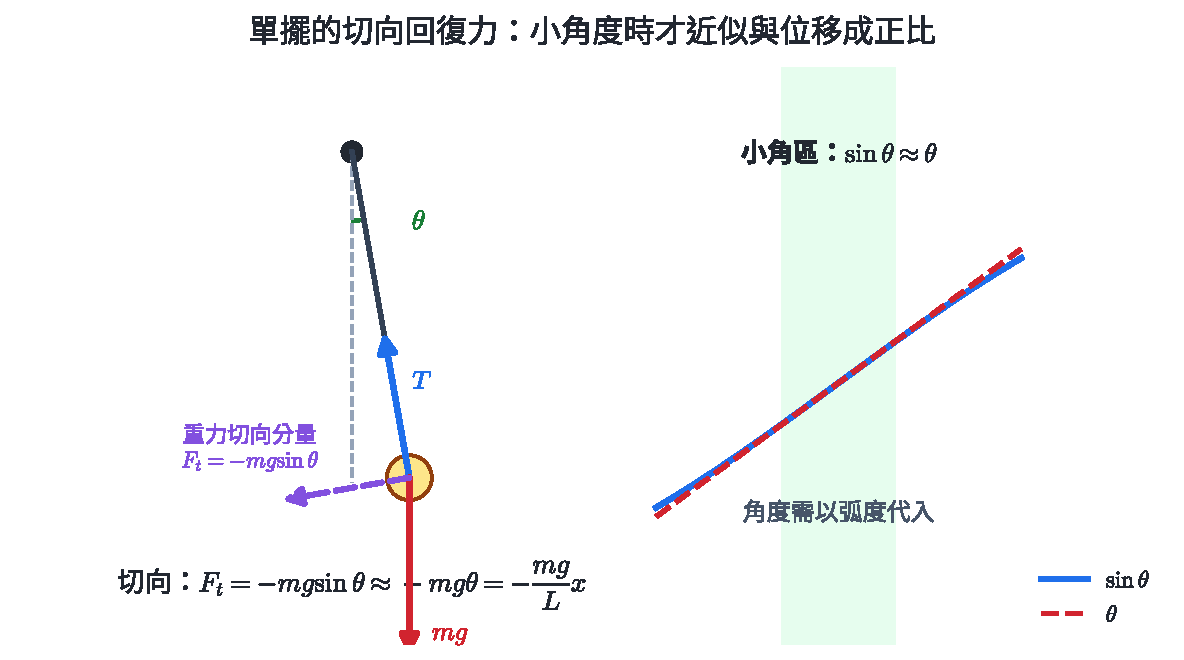
\includegraphics[width=0.94\linewidth,height=\textheight,keepaspectratio,alt={圖 7A｜紫色虛線是重力的切向分量 F\_t=-mg\textbackslash sin\textbackslash theta；圖中擺角 10\^{}\textbackslash circ 落在小角區。當 \textbackslash theta 以弧度表示且角度小，\textbackslash sin\textbackslash theta\textbackslash approx\textbackslash theta=x/L。}]{assets/選物I-4-單擺小角度.pdf}
\caption{圖 7A｜紫色虛線是重力的切向分量 \(F_t=-mg\sin\theta\)；圖中擺角 \(10^\circ\) 落在小角區。當 \(\theta\) 以弧度表示且角度小，\(\sin\theta\approx\theta=x/L\)。}
\end{figure}

長度 \(L\) 的單擺，切向回復力為 \(-mg\sin\theta\)。小角度且以弧度表示時，\(\sin\theta\approx\theta\)，弧長 \(x=L\theta\)，因此

\[
F_t\approx-mg\frac{x}{L}.
\]

形式與 \(-kx\) 相同，所以小角度單擺近似簡諧，週期為

\[
\boxed{T=2\pi\sqrt{\frac{L}{g}}}.
\]

週期與擺球質量無關；小角度近似下也近似不依振幅。角度大時 \(\sin\theta\approx\theta\) 失效，週期會偏離此式。

\subsection{擺鐘週期與重力測量取決於擺長}\label{ux64faux9418ux9031ux671fux8207ux91cdux529bux6e2cux91cfux53d6ux6c7aux65bcux64faux9577}

\(T\propto\sqrt L\)，所以改變有效擺長就能調整走時。由於 \(T\propto1/\sqrt g\)，不同地點的重力加速度差異會使同一擺鐘產生微小走時差。反過來，精確量得 \(L,T\) 後可由 \(g=4\pi^2L/T^2\) 估計當地 \(g\)，但須控制振幅、空氣阻力、支點摩擦與長度定義。

\begin{HandoutWorkedExample}

\subsection{完整示範｜擺長對週期的影響}\label{ux5b8cux6574ux793aux7bc4ux64faux9577ux5c0dux9031ux671fux7684ux5f71ux97ff}

\(L=0.81\ \mathrm m\)，取 \(g=10\ \mathrm{m/s^2}\)：

\[
T=2\pi\sqrt{\frac{0.81}{10}}
\approx1.79\ \mathrm s.
\]

若擺長增為 \(4L\)，

\[
\frac{T'}T=\sqrt{\frac{4L}{L}}=2,
\]

新週期約 \(3.58\ \mathrm s\)。

\end{HandoutWorkedExample}

\begin{HandoutWorkedExample}

\subsection{\texorpdfstring{完整示範｜由擺長與週期估計 \(g\)}{完整示範｜由擺長與週期估計 g}}\label{ux5b8cux6574ux793aux7bc4ux7531ux64faux9577ux8207ux9031ux671fux4f30ux8a08-g}

擺長 \(L=0.640\ \mathrm m\)，小角度測得週期 \(T=1.60\ \mathrm s\)。

\[
g=\frac{4\pi^2L}{T^2}
=\frac{4\pi^2(0.640)}{1.60^2}
=\pi^2
\approx9.87\ \mathrm{m/s^2}.
\]

擺長由懸點量到擺球質心。實驗可量 10 或 20 週總時間後再除以週數，降低單次按表反應時間的影響。

\end{HandoutWorkedExample}

\begin{HandoutSelfCheck}

\subsection{練習｜小角度單擺}\label{ux7df4ux7fd2ux5c0fux89d2ux5ea6ux55aeux64fa}

\begin{enumerate}
\def\labelenumi{\arabic{enumi}.}
\tightlist
\item
  \(L=1.00\ \mathrm m\)、\(g=9.8\ \mathrm{m/s^2}\)，求週期。
\item
  擺球質量加倍，擺長不變，比較週期。
\item
  週期要增為 3 倍，擺長要變為幾倍？
\item
  大擺角資料比小角度公式預測的週期略長。指出推導中已偏離實際的近似步驟。
\end{enumerate}

\textbf{簡答：}1. 約 \(2.01\ \mathrm s\)。2. 不變。3. 9 倍。4. \(\sin\theta\approx\theta\) 的小角度近似已不足。

\end{HandoutSelfCheck}

\section{8. 一頁核心整理}\label{ux4e00ux9801ux6838ux5fc3ux6574ux7406}

\subsection{三大定律與解題骨架}\label{ux4e09ux5927ux5b9aux5f8bux8207ux89e3ux984cux9aa8ux67b6}

\begin{itemize}
\tightlist
\item
  第一：\(\sum\vec F=0\Rightarrow\vec v\) 為常向量。
\item
  第二：\(\sum\vec F=m\vec a\)；先畫自由體圖，再逐分量列式。
\item
  第三：\(\vec F_{A\to B}=-\vec F_{B\to A}\)；兩力在不同物體。
\item
  虎克：比例限度內 \(\vec F_s=-k\vec x\)。
\end{itemize}

\subsection{圓周}\label{ux5713ux5468}

\[
\omega_{\mathrm{speed}}=2\pi f=\frac{2\pi}{T},
\quad
v=R|\omega|,
\quad
a_c=\frac{v^2}{R}=R\omega^2,
\quad
\sum F_r=ma_c.
\]

向心力是徑向合力的角色，不另畫成一種力。

\subsection{簡諧}\label{ux7c21ux8ae7}

\[
a=-\omega^2x,
\quad
x=A\cos\omega t,
\quad
T=\frac{2\pi}{\omega}.
\]

彈簧：\(\omega=\sqrt{k/m}\)、\(T=2\pi\sqrt{m/k}\)。小角度單擺：\(T=2\pi\sqrt{L/g}\)。

\section{9. 代表題：分層練習}\label{ux4ee3ux8868ux984cux5206ux5c64ux7df4ux7fd2}

\subsection{題目 1｜力的分量與合成}\label{ux984cux76ee-1ux529bux7684ux5206ux91cfux8207ux5408ux6210}

一物體同時受 \(10\ \mathrm N\) 向東與 \(10\ \mathrm N\) 北偏西 \(60^\circ\) 的力。先畫向量分量圖，再求合力分量與量值。

\subsection{題目 2｜虎克定律}\label{ux984cux76ee-2ux864eux514bux5b9aux5f8b}

彈簧自然長 \(20\ \mathrm{cm}\)，受 \(6.0\ \mathrm N\) 拉力後長 \(23\ \mathrm{cm}\)。在比例限度內，求 \(k\)；若壓縮至 \(18\ \mathrm{cm}\)，彈簧作用力的量值與方向為何？

\subsection{題目 3｜斜面與自由體圖}\label{ux984cux76ee-3ux659cux9762ux8207ux81eaux7531ux9ad4ux5716}

\(3.0\ \mathrm{kg}\) 物體在 \(30^\circ\) 光滑斜面上自由滑下，取 \(g=10\ \mathrm{m/s^2}\)。由自由體圖判斷應採「沿斜面／垂直斜面」或「水平／鉛直」分量較直接，再求沿斜面加速度與正向力。

\subsection{題目 4｜第三定律辨析}\label{ux984cux76ee-4ux7b2cux4e09ux5b9aux5f8bux8fa8ux6790}

書靜止在桌上。畫出書、桌面、地球三個節點，以箭頭連出兩組交互作用；標明「地球對書的重力」與「桌面對書的正向力」各自的第三定律配對，並說明書上的兩力為何不是一對作用反作用力。

\subsection{題目 5｜連接體}\label{ux984cux76ee-5ux9023ux63a5ux9ad4}

光滑水平面上，\(2.0\ \mathrm{kg}\) 木塊在左、\(3.0\ \mathrm{kg}\) 木塊在右並彼此接觸。以水平 \(20\ \mathrm N\) 向右推左側木塊，求共同加速度與接觸力量值；若改以同樣的力向右推右側木塊，比較共同加速度與接觸力量值。

\subsection{題目 6｜視重}\label{ux984cux76ee-6ux8996ux91cd}

質量 \(60\ \mathrm{kg}\) 的人站在電梯秤上，取向上為正。速度感測器顯示 \(t=0\) 時 \(v_y=+4.0\ \mathrm{m/s}\)，\(t=0.50\ \mathrm s\) 時 \(v_y=+3.0\ \mathrm{m/s}\)，區間內加速度近似固定。取 \(g=10\ \mathrm{m/s^2}\)，求秤的正向力。

\subsection{題目 7｜等速圓周}\label{ux984cux76ee-7ux7b49ux901fux5713ux5468}

\(0.25\ \mathrm{kg}\) 小球在 \(5.0\ \mathrm s\) 內逆時針完成 10 圈，圓周半徑為 \(0.50\ \mathrm m\)。取逆時針角位移為正，求帶符號角速度、線速率、向心加速度與徑向合力量值。

\subsection{題目 8｜簡諧運動}\label{ux984cux76ee-8ux7c21ux8ae7ux904bux52d5}

\(0.50\ \mathrm{kg}\) 物體連接 \(k=200\ \mathrm{N/m}\) 的理想彈簧，在光滑水平面作振幅 \(0.040\ \mathrm m\) 的振動；實測週期為 \(0.320\ \mathrm s\)。選用理想簡諧模型求角頻率、理論週期、最大速率與最大加速度，並計算實測週期相對理論值的百分差。

\subsection{題目 9｜小角度單擺與範圍}\label{ux984cux76ee-9ux5c0fux89d2ux5ea6ux55aeux64faux8207ux7bc4ux570d}

同一支長 \(1.00\ \mathrm m\) 的單擺先後換上 \(0.10\ \mathrm{kg}\)、\(0.20\ \mathrm{kg}\) 擺球，小角度量得週期均約 \(2.0\ \mathrm s\)；改用同一擺球作大擺角運動時，週期略增。取 \(g=9.8\ \mathrm{m/s^2}\)，用小角模型估計週期，並判斷兩組資料分別支持或偏離模型的哪一項前提。

\subsection{題目 10｜牛頓第二定律實驗}\label{ux984cux76ee-10ux725bux9813ux7b2cux4e8cux5b9aux5f8bux5be6ux9a57}

固定系統質量時，實驗最佳直線為 \(a=0.32F_{\mathrm{net}}+0.05\)（SI 單位）。求斜率對應的系統質量，並解釋截距的物理意義。

\subsection{題目 11｜電梯視重}\label{ux984cux76ee-11ux96fbux68afux8996ux91cd}

\(55\ \mathrm{kg}\) 人在電梯中，秤讀值對應 \(N=440\ \mathrm N\)，取 \(g=10\ \mathrm{m/s^2}\)。求加速度。若電梯當時向下運動，判斷速率增減。

\subsection{題目 12｜阿特伍德機}\label{ux984cux76ee-12ux963fux7279ux4f0dux5fb7ux6a5f}

理想滑輪兩側懸掛 \(3.0\ \mathrm{kg}\) 與 \(5.0\ \mathrm{kg}\)，取 \(g=10\ \mathrm{m/s^2}\)。畫兩物體受力圖，求加速度與繩張力。

\subsection{題目 13｜鉛直圓底端}\label{ux984cux76ee-13ux925bux76f4ux5713ux5e95ux7aef}

\(0.50\ \mathrm{kg}\) 物體在 \(R=1.0\ \mathrm m\) 的鉛直圓軌道底端速率為 \(5.0\ \mathrm{m/s}\)，取 \(g=10\ \mathrm{m/s^2}\)。畫受力圖並求軌道對物體的正向力。

\subsection{題目 14｜簡諧相位}\label{ux984cux76ee-14ux7c21ux8ae7ux76f8ux4f4d}

簡諧物體滿足 \(x=0.10\cos(4t)\)（SI 單位）。求 \(t=\pi/8\ \mathrm s\) 時的 \(x\)、\(v\)、\(a\)，並在相位圖上指出該時刻。

\subsection{題目 15｜單擺資料}\label{ux984cux76ee-15ux55aeux64faux8cc7ux6599}

小角度單擺實驗得到下表。以通過原點的 \(T^2\)--\(L\) 最佳線斜率約 \(4.01\ \mathrm{s^2/m}\)，由模型估計 \(g\)，並指出量測多週總時間再除以週數的目的。

{\def\LTcaptype{none} % do not increment counter
\begin{longtable}[]{@{}rrrr@{}}
\toprule\noalign{}
\(L\)（m） & \(0.40\) & \(0.60\) & \(0.80\) \\
\midrule\noalign{}
\endhead
\bottomrule\noalign{}
\endlastfoot
\(T\)（s） & \(1.27\) & \(1.55\) & \(1.79\) \\
\end{longtable}
}

\subsection{整合題 1｜斜面連接體}\label{ux6574ux5408ux984c-1ux659cux9762ux9023ux63a5ux9ad4}

兩個物塊 \(m_1=2.0\ \mathrm{kg}\)、\(m_2=3.0\ \mathrm{kg}\) 在同一 \(30^\circ\) 光滑斜面上以輕繩前後相連。\(35\ \mathrm N\) 力沿斜面向上拉前方 \(m_2\)。取 \(g=10\ \mathrm{m/s^2}\)，畫兩個受力圖，求共同加速度與繩張力。

\subsection{整合題 2｜彈簧提供向心合力}\label{ux6574ux5408ux984c-2ux5f48ux7c27ux63d0ux4f9bux5411ux5fc3ux5408ux529b}

\(0.40\ \mathrm{kg}\) 小球連接自然長 \(0.50\ \mathrm m\)、\(k=80\ \mathrm{N/m}\) 的彈簧，在光滑水平面上以半徑 \(0.60\ \mathrm m\) 繞圓。彈簧沿半徑方向指向圓心。求彈簧力與小球速率。

\subsection{整合題 3｜電梯內的彈簧秤}\label{ux6574ux5408ux984c-3ux96fbux68afux5167ux7684ux5f48ux7c27ux79e4}

\(2.0\ \mathrm{kg}\) 物體懸掛在 \(k=500\ \mathrm{N/m}\) 彈簧下端，與電梯相對靜止。電梯以 \(2.0\ \mathrm{m/s^2}\) 向上加速，取 \(g=10\ \mathrm{m/s^2}\)。畫物體受力圖，求彈簧伸長量。

\subsection{整合題 4｜簡諧運動感測數據}\label{ux6574ux5408ux984c-4ux7c21ux8ae7ux904bux52d5ux611fux6e2cux6578ux64da}

感測器測得某振動系統在 \(t=0\)、\(0.20\)、\(0.40\)、\(0.60\)、\(0.80\ \mathrm s\) 的位移分別為 \(+4.0\)、0、\(-4.0\)、0、\(+4.0\ \mathrm{cm}\)。建立無初相的 cosine 模型，求 \(\omega\)、\(v_{\max}\)，並預測 \(t=0.10\ \mathrm s\) 的位移。

\clearpage

\section{10. 完整解析}\label{ux5b8cux6574ux89e3ux6790}

\begin{figure}
\centering
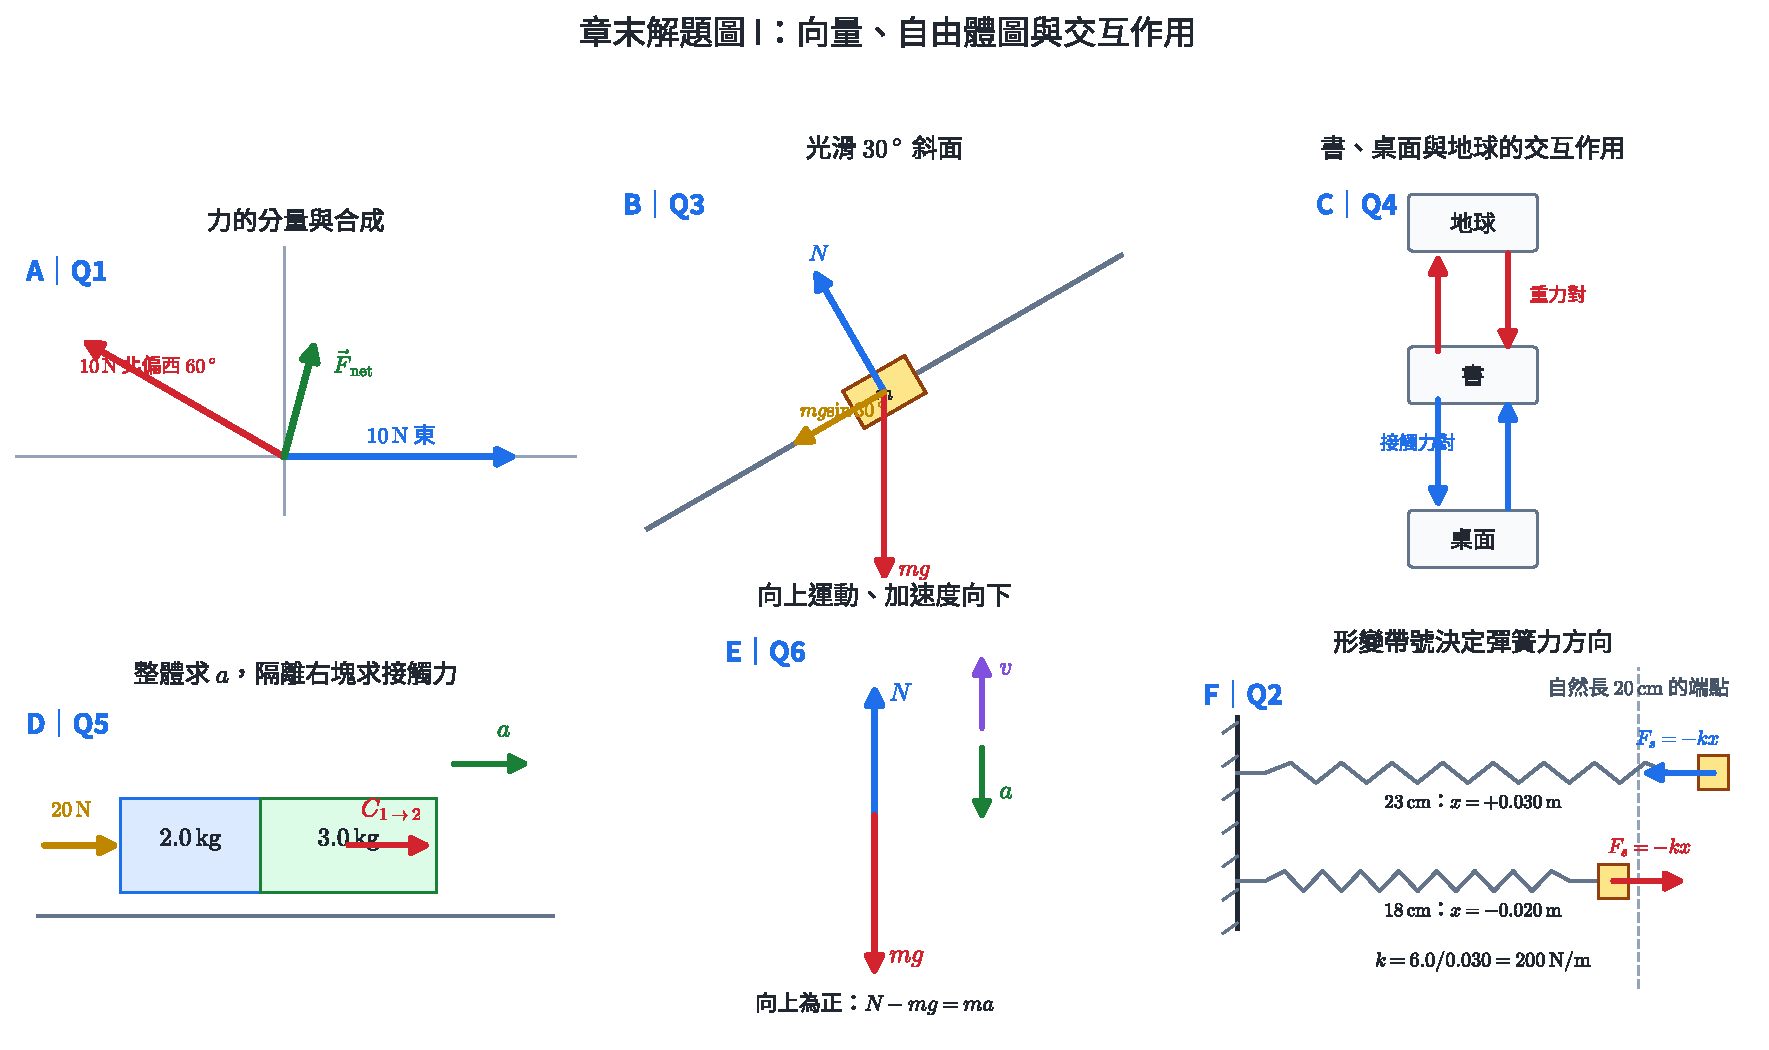
\includegraphics[width=0.98\linewidth,height=\textheight,keepaspectratio,alt={解題圖 A｜panel A--F 對應第 1--6 題；箭頭、坐標與彈簧形變方向直接決定分量及方程正負號。}]{assets/選物I-4-章末受力解題圖.pdf}
\caption{解題圖 A｜panel A--F 對應第 1--6 題；箭頭、坐標與彈簧形變方向直接決定分量及方程正負號。}
\end{figure}

\subsection{第 1 題}\label{ux7b2c-1-ux984c}

依解題圖 A 的 panel A，取東、北為正。第二力北偏西 \(60^\circ\)，西向分量大小 \(10\sin60^\circ=5\sqrt3\)，北向分量 \(10\cos60^\circ=5\)：

\[
F_x=10-5\sqrt3,
\qquad
F_y=5.
\]

合力量值

\[
F=\sqrt{(10-5\sqrt3)^2+5^2}\approx5.18\ \mathrm N.
\]

\subsection{第 2 題}\label{ux7b2c-2-ux984c}

依解題圖 A 的 panel F，令伸長為正；\(23\ \mathrm{cm}\) 對應 \(x=+0.030\ \mathrm m\)：

\[
k=\frac{6.0}{0.030}=200\ \mathrm{N/m}.
\]

壓縮至 \(18\ \mathrm{cm}\) 時 \(x=-0.020\ \mathrm m\)。由 panel F 的箭頭與 \(F_s=-kx\)，力指向正方向，量值為 \(k|x|=4.0\ \mathrm N\)；即把受力端向外推回自然長度。

\subsection{第 3 題}\label{ux7b2c-3-ux984c}

解題圖 A 的 panel B 使兩支力各只有一個方向需要分解，因此採沿斜面與垂直斜面的座標較直接。物體受重力 \(mg\) 向下與正向力 \(N\) 垂直接觸面。沿斜面：

\[
mg\sin30^\circ=ma
\Rightarrow a=g\sin30^\circ=5.0\ \mathrm{m/s^2}.
\]

垂直斜面沒有加速度：

\[
N=mg\cos30^\circ=30\left(\frac{\sqrt3}{2}\right)=15\sqrt3\ \mathrm N.
\]

\subsection{第 4 題}\label{ux7b2c-4-ux984c}

解題圖 A 的 panel C 以一條連線表示一組交互作用，連線兩端的反向箭頭就是第三定律力對：

\begin{itemize}
\tightlist
\item
  地球對書的重力，配對為書對地球的萬有引力。
\item
  桌面對書的正向力，配對為書對桌面的接觸力。
\end{itemize}

重力與正向力都作用在書上；在此靜止且僅有兩力的情境中兩者等大反向、合力為 0。第三定律力對必作用在不同物體，且來自同一交互作用。

\subsection{第 5 題}\label{ux7b2c-5-ux984c}

依解題圖 A 的 panel D，先把兩塊視為整體，總質量 \(5.0\ \mathrm{kg}\)：

\[
a=\frac{20}{5.0}=4.0\ \mathrm{m/s^2}.
\]

隔離 \(3.0\ \mathrm{kg}\) 木塊，它的水平合力只有前一塊的接觸力，所以

\[
F_c=(3.0)(4.0)=12\ \mathrm N.
\]

改推右側木塊時，外力與總質量不變，所以共同加速度仍為 \(4.0\ \mathrm{m/s^2}\)；此時隔離左側 \(2.0\ \mathrm{kg}\) 木塊，接觸力為

\[
F_c=(2.0)(4.0)=8.0\ \mathrm N.
\]

接觸力取決於它需要加速哪一部分系統，因此兩種推法的接觸力不同。

\subsection{第 6 題}\label{ux7b2c-6-ux984c}

由速度資料先求

\[
a=\frac{3.0-4.0}{0.50}=-2.0\ \mathrm{m/s^2}.
\]

依解題圖 A 的 panel E，速度向上而加速度向下；取向上為正：

\[
N-mg=ma
\Rightarrow
N=m(g+a)=60(10-2)=480\ \mathrm N.
\]

視重小於實重。速度方向不直接決定秤讀數。

\subsection{第 7 題}\label{ux7b2c-7-ux984c}

\begin{figure}
\centering
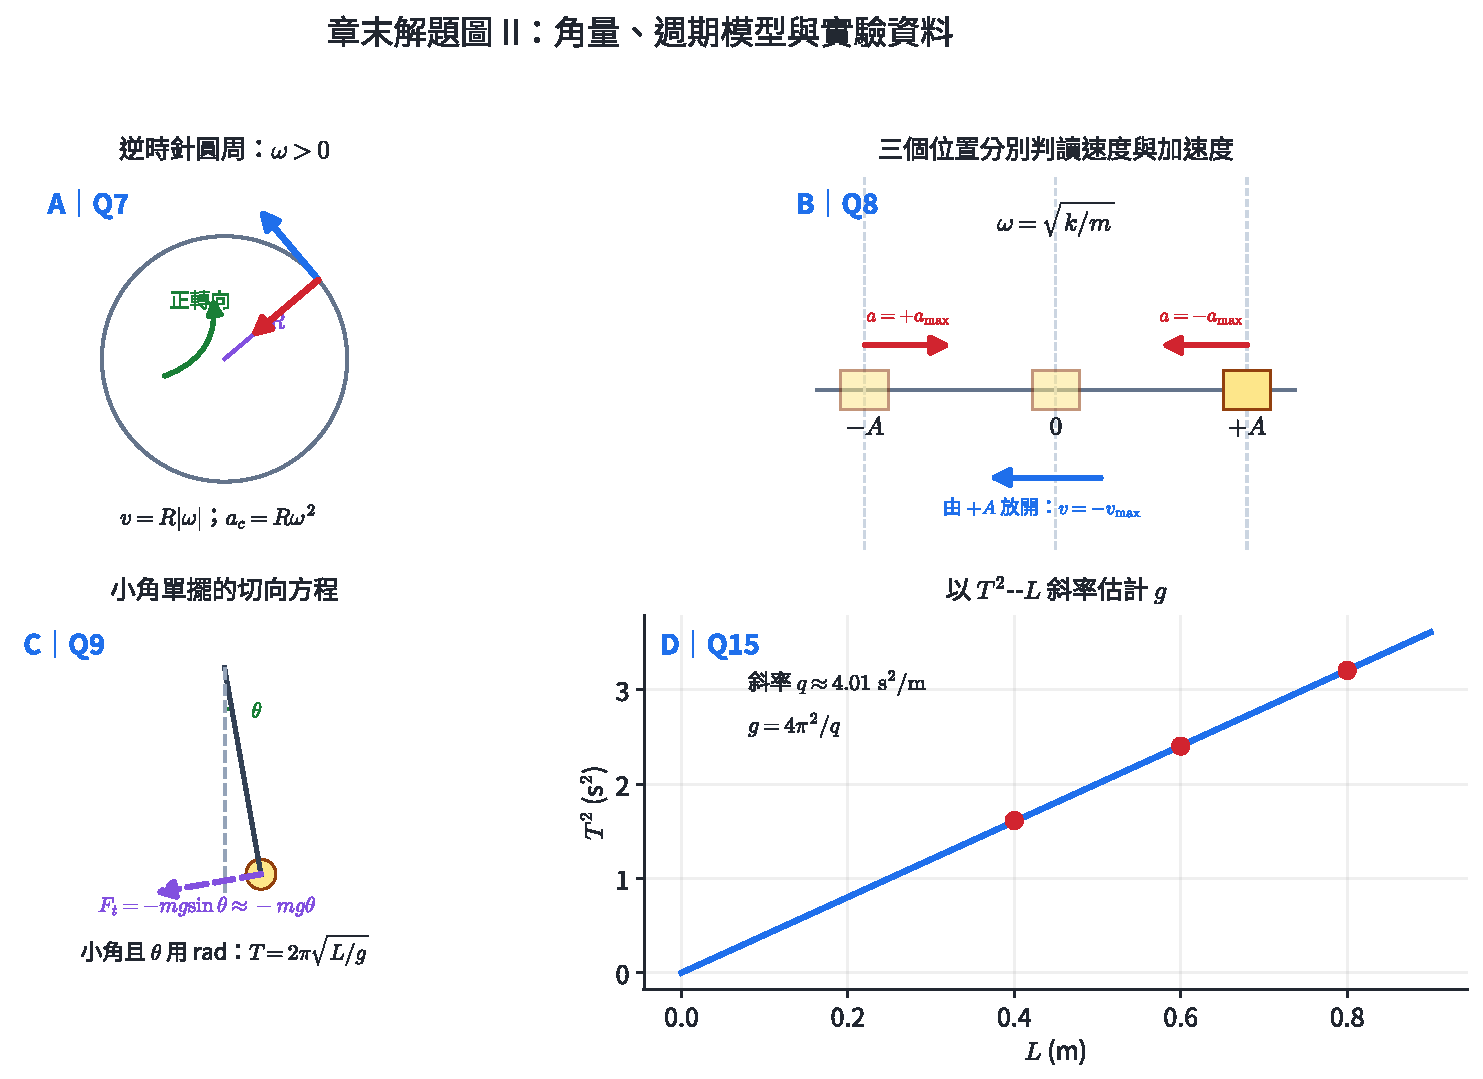
\includegraphics[width=0.98\linewidth,height=\textheight,keepaspectratio,alt={解題圖 B｜panel A--D 分別對應第 7、8、9、15 題；方向、極值位置、模型前提與實驗斜率都直接進入列式。}]{assets/選物I-4-章末週期解題圖.pdf}
\caption{解題圖 B｜panel A--D 分別對應第 7、8、9、15 題；方向、極值位置、模型前提與實驗斜率都直接進入列式。}
\end{figure}

觀測頻率為 \(f=10/5.0=2.0\ \mathrm{Hz}\)。依解題圖 B 的 panel A，逆時針為正，所以

\[
\omega=2\pi f=4\pi\ \mathrm{rad/s},
\]

\[
v=R\omega=(0.50)(4\pi)=2\pi\ \mathrm{m/s},
\]

\[
a_c=R\omega^2=(0.50)(4\pi)^2=8\pi^2\ \mathrm{m/s^2},
\]

\[
F_r=ma_c=(0.25)(8\pi^2)=2\pi^2\ \mathrm N.
\]

方向皆針對徑向量：加速度與合力指向圓心。

\subsection{第 8 題}\label{ux7b2c-8-ux984c}

依解題圖 B 的 panel B，端點給最大加速度量值，平衡點給最大速率。理想模型先給

\[
\omega=\sqrt{\frac{k}{m}}=\sqrt{\frac{200}{0.50}}=20\ \mathrm{rad/s},
\]

\[
T=\frac{2\pi}{20}=\frac{\pi}{10}\ \mathrm s\approx0.314\ \mathrm s.
\]

\[
v_{\max}=A\omega=(0.040)(20)=0.80\ \mathrm{m/s},
\]

\[
a_{\max}=A\omega^2=(0.040)(400)=16\ \mathrm{m/s^2}.
\]

實測週期相對理論值的百分差為

\[
\frac{|0.320-0.314|}{0.314}\times100\%\approx1.9\%.
\]

\subsection{第 9 題}\label{ux7b2c-9-ux984c}

解題圖 B 的 panel C 顯示小角模型使用 \(\sin\theta\approx\theta\)，且 \(\theta\) 以弧度表示：

\[
T=2\pi\sqrt{\frac{1.00}{9.8}}\approx2.01\ \mathrm s.
\]

公式不含擺球質量，兩種質量測得相同週期支持「理想週期與擺球質量無關」。大擺角資料的週期增加，表示 \(\sin\theta\approx\theta\) 已不足，運動不再是嚴格簡諧。

\subsection{第 10--12 題的圖像與受力圖}\label{ux7b2c-1012-ux984cux7684ux5716ux50cfux8207ux53d7ux529bux5716}

\begin{figure}
\centering
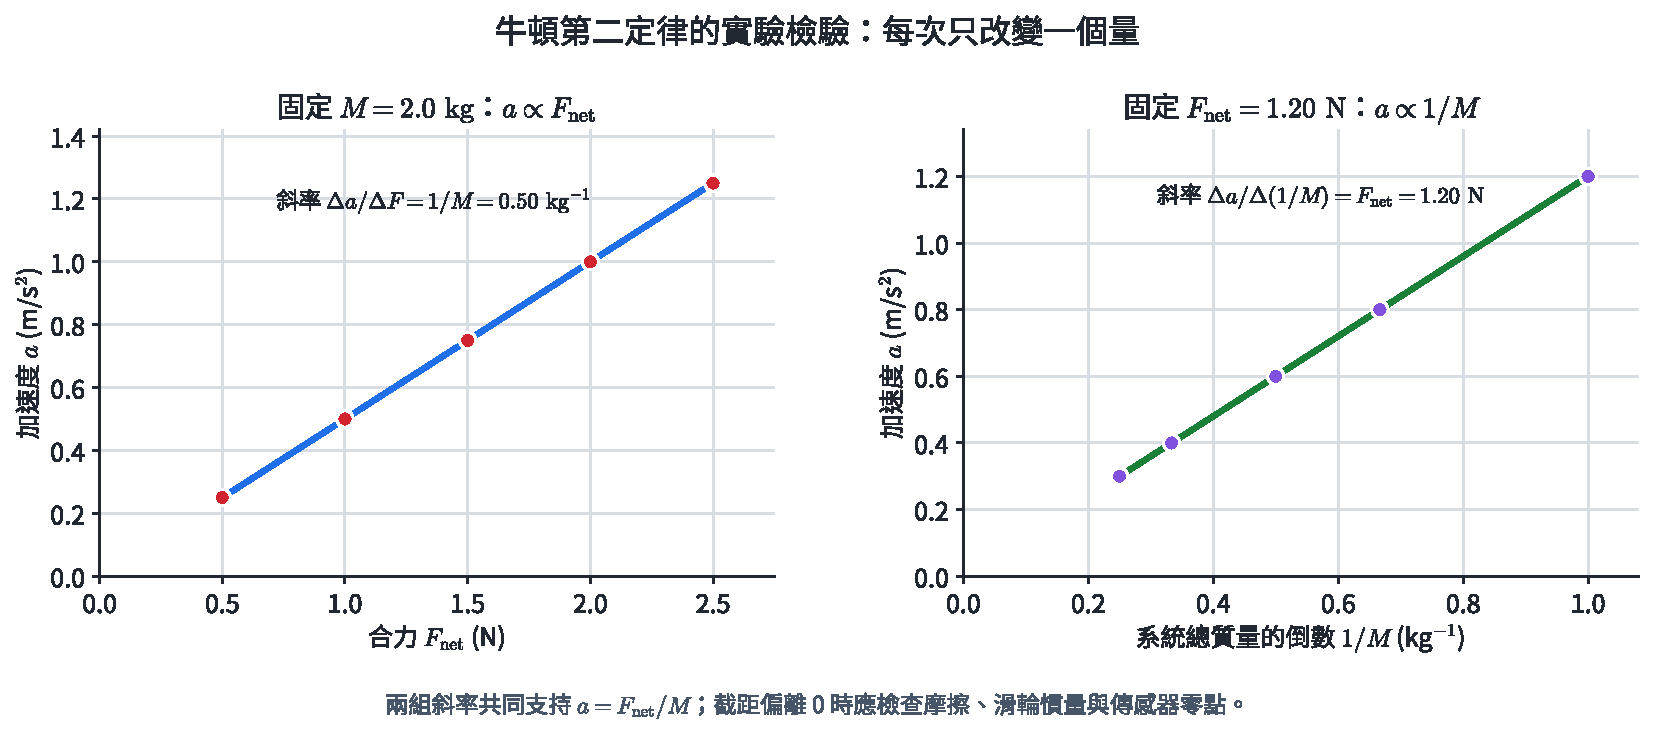
\includegraphics[width=0.94\linewidth,height=\textheight,keepaspectratio,alt={解題圖 A｜實驗圖的斜率對應 1/m 或 F\_\{\textbackslash mathrm\{net\}\}，截距用來辨識未納入的恆定效應。}]{assets/選物I-4-牛頓第二定律實驗.pdf}
\caption{解題圖 A｜實驗圖的斜率對應 \(1/m\) 或 \(F_{\mathrm{net}}\)，截距用來辨識未納入的恆定效應。}
\end{figure}

\begin{figure}
\centering
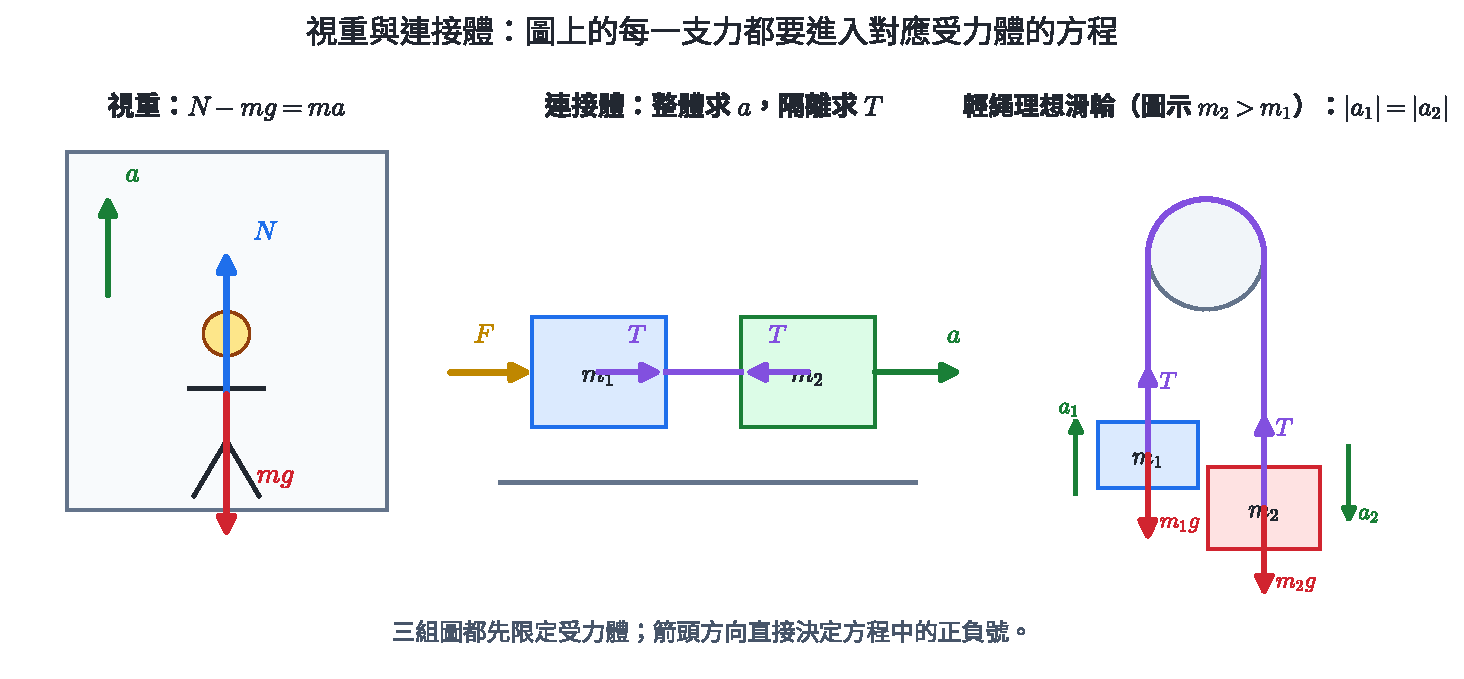
\includegraphics[width=0.96\linewidth,height=\textheight,keepaspectratio,alt={解題圖 B｜電梯與阿特伍德機中，箭頭方向直接決定方程正負號。}]{assets/選物I-4-視重與連接體.pdf}
\caption{解題圖 B｜電梯與阿特伍德機中，箭頭方向直接決定方程正負號。}
\end{figure}

\subsection{第 10 題}\label{ux7b2c-10-ux984c}

\(a\) 對 \(F_{\mathrm{net}}\) 圖的斜率為 \(1/m\)：

\[
\frac1m=0.32\ \mathrm{kg^{-1}}
\quad\Rightarrow\quad
m=3.125\ \mathrm{kg}\approx3.1\ \mathrm{kg}.
\]

截距 \(0.05\ \mathrm{m/s^2}\) 表示圖線在設定合力為 0 時仍預測非零加速度。可檢查感測器零點、桌面微傾或合力未完整扣除摩擦。

\subsection{第 11 題}\label{ux7b2c-11-ux984c}

依解題圖 B 左圖，取向上為正：

\[
N-mg=ma,
\]

\[
440-550=55a
\Rightarrow a=-2.0\ \mathrm{m/s^2}.
\]

加速度向下。電梯當下也向下運動，速度與加速度同向，所以速率增加。

\subsection{第 12 題}\label{ux7b2c-12-ux984c}

依解題圖 B 右圖，\(5.0\ \mathrm{kg}\) 向下為正，\(3.0\ \mathrm{kg}\) 向上為正：

\[
5g-T=5a,
\qquad
T-3g=3a.
\]

相加得

\[
a=\frac{5-3}{5+3}g=2.5\ \mathrm{m/s^2}.
\]

代回較輕一側：

\[
T=3(g+a)=3(10+2.5)=37.5\ \mathrm N.
\]

張力量值介於 \(3g=30\ \mathrm N\) 與 \(5g=50\ \mathrm N\) 之間；同一輕繩兩端張力量值相同，方向各沿繩拉離受力體。

\subsection{第 13--15 題的圓周、相位與單擺圖}\label{ux7b2c-1315-ux984cux7684ux5713ux5468ux76f8ux4f4dux8207ux55aeux64faux5716}

\begin{figure}
\centering
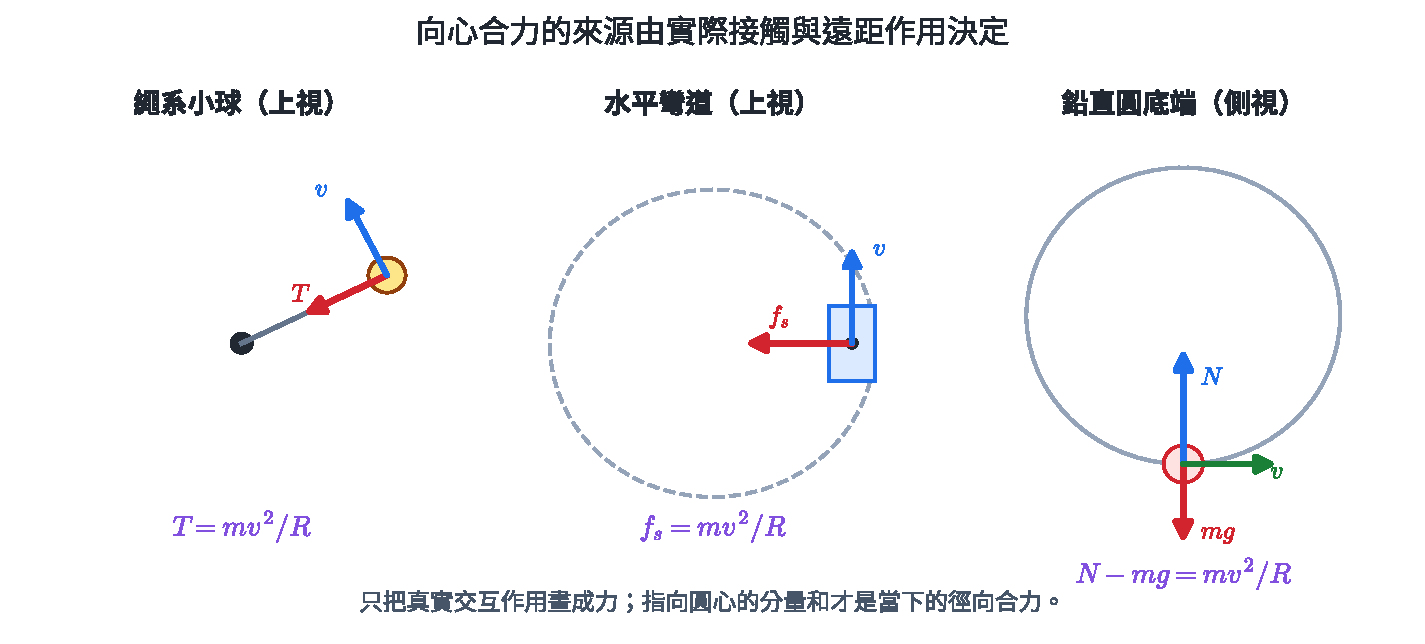
\includegraphics[width=0.94\linewidth,height=\textheight,keepaspectratio,alt={解題圖 C｜鉛直圓底端的正向力向上、重力向下，徑向合力指向圓心。}]{assets/選物I-4-圓周受力模型.pdf}
\caption{解題圖 C｜鉛直圓底端的正向力向上、重力向下，徑向合力指向圓心。}
\end{figure}

\begin{figure}
\centering
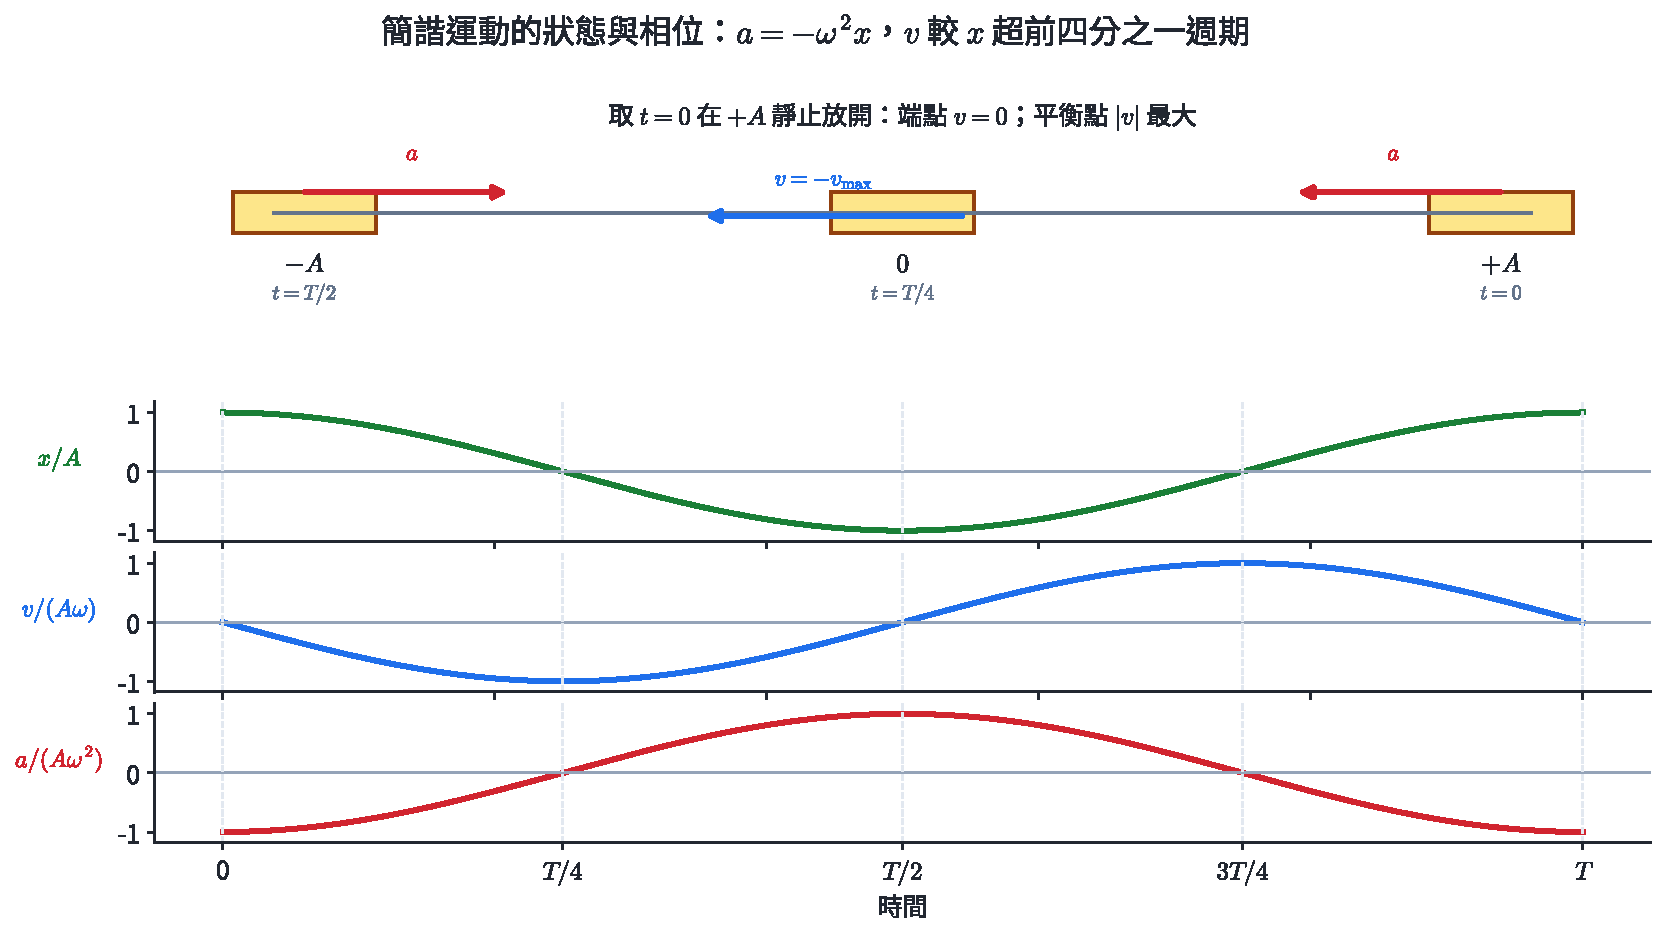
\includegraphics[width=0.96\linewidth,height=\textheight,keepaspectratio,alt={解題圖 D｜簡諧運動的 x、v、a 相位圖與單擺小角度受力圖。}]{assets/選物I-4-簡諧狀態與相位.pdf}
\caption{解題圖 D｜簡諧運動的 \(x\)、\(v\)、\(a\) 相位圖與單擺小角度受力圖。}
\end{figure}

\subsection{第 13 題}\label{ux7b2c-13-ux984c}

解題圖 C 的底端圓心向上；\(N\) 向上，\(mg\) 向下：

\[
N-mg=m\frac{v^2}{R}.
\]

\[
N=mg+m\frac{v^2}{R}
=(0.50)(10)+(0.50)\frac{25}{1.0}
=17.5\ \mathrm N.
\]

\subsection{第 14 題}\label{ux7b2c-14-ux984c}

\(t=\pi/8\ \mathrm s\) 時，\(\omega t=4(\pi/8)=\pi/2\)，對應解題圖 D 的 \(T/4\)：

\[
x=0.10\cos\frac\pi2=0,
\]

\[
v=-(0.10)(4)\sin\frac\pi2=-0.40\ \mathrm{m/s},
\]

\[
a=-\omega^2x=0.
\]

物體由正端點穿越平衡點，速度向 \(-x\)。

\subsection{第 15 題}\label{ux7b2c-15-ux984c}

由 \(T=2\pi\sqrt{L/g}\) 平方得 \(T^2=(4\pi^2/g)L\)。依解題圖 B 的 panel D，最佳線斜率 \(q=4.01\ \mathrm{s^2/m}\)，所以

\[
g=\frac{4\pi^2}{q}
=\frac{4\pi^2}{4.01}
\approx9.84\ \mathrm{m/s^2}.
\]

量多週總時間再除以週數，可把一次啟停的反應時間誤差分攤到多個週期。結果仍受擺長定義、振幅、阻力與圖線擬合影響。

\subsection{整合題的建模圖}\label{ux6574ux5408ux984cux7684ux5efaux6a21ux5716}

\begin{figure}
\centering
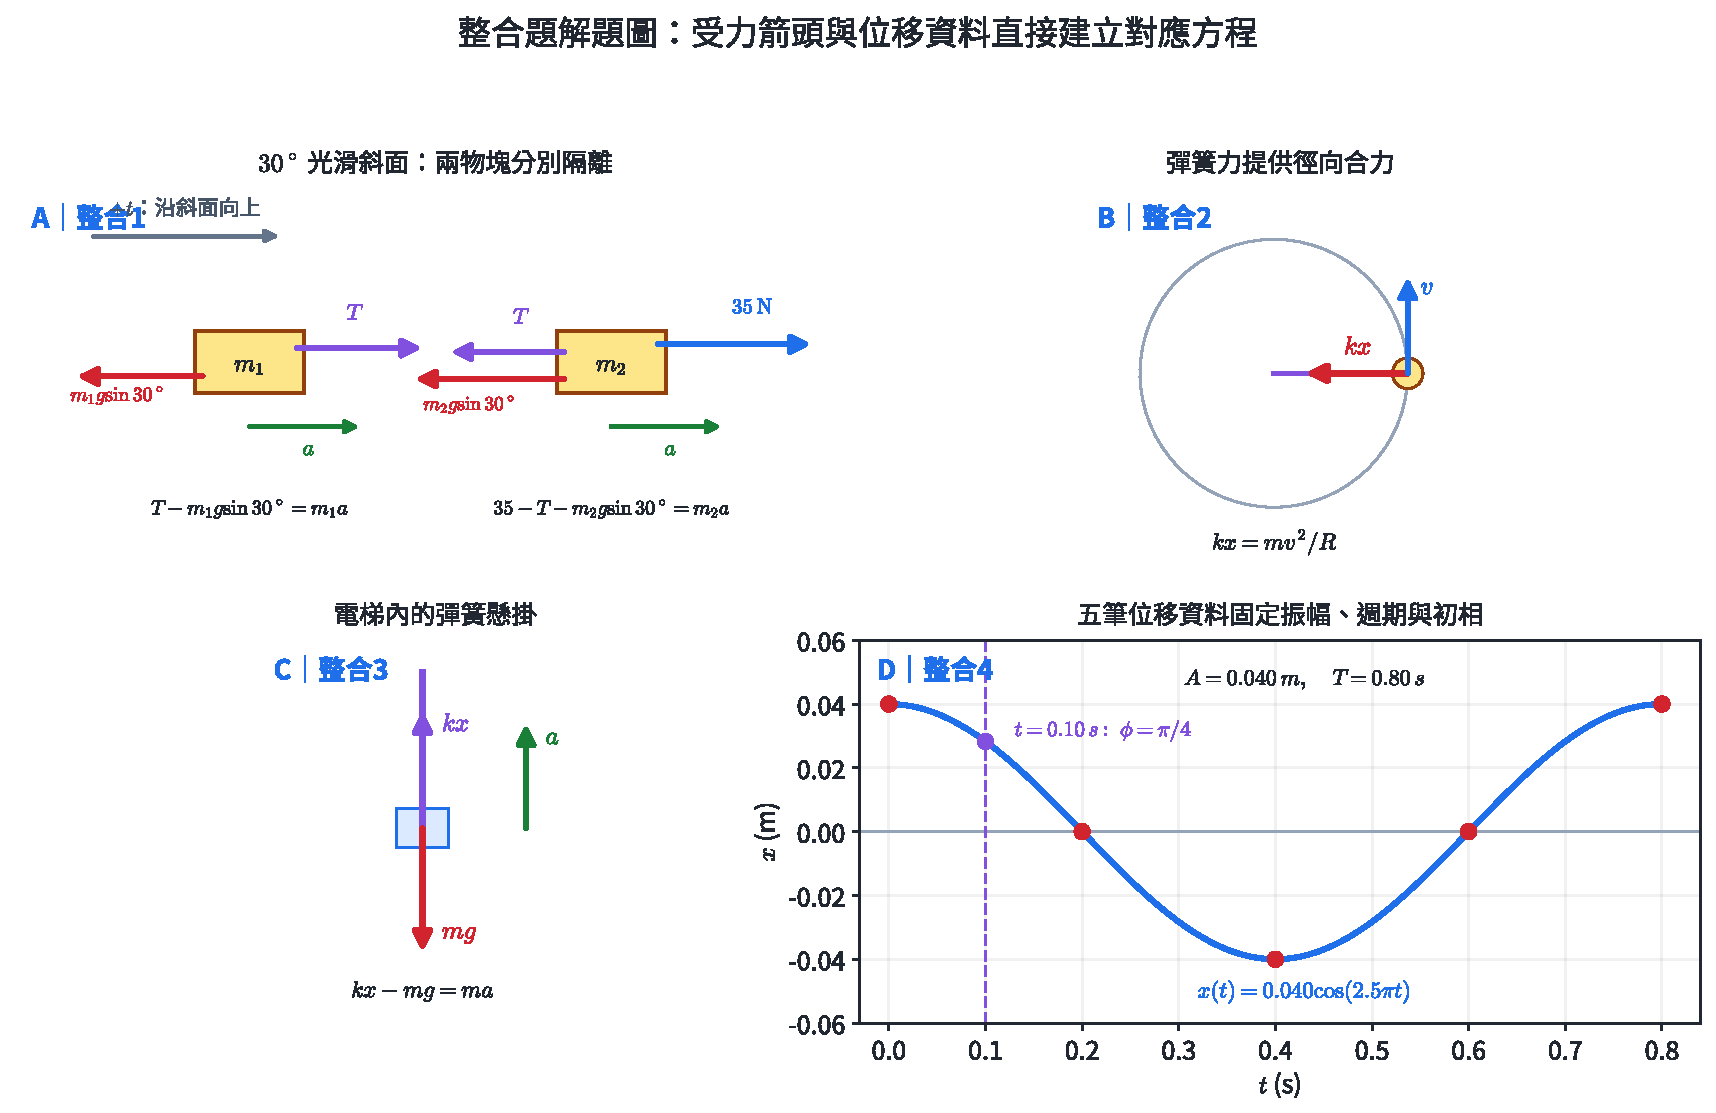
\includegraphics[width=0.98\linewidth,height=\textheight,keepaspectratio,alt={解題圖 C｜panel A 把 m\_1、m\_2 分別隔離，統一以沿斜面向上為正，箭頭直接對應兩條沿斜面方程；panel B、C 建立徑向與鉛直受力式，panel D 由五筆位移資料建立振幅、週期與初相。}]{assets/選物I-4-整合題解題圖.pdf}
\caption{解題圖 C｜panel A 把 \(m_1\)、\(m_2\) 分別隔離，統一以沿斜面向上為正，箭頭直接對應兩條沿斜面方程；panel B、C 建立徑向與鉛直受力式，panel D 由五筆位移資料建立振幅、週期與初相。}
\end{figure}

\subsection{整合題 1}\label{ux6574ux5408ux984c-1}

依解題圖 C 的 panel A，兩物塊都受重力、正向力；\(m_1\) 受張力向上，\(m_2\) 受張力向下並受 \(35\ \mathrm N\) 向上。把兩物塊視為整體：

\[
35-(m_1+m_2)g\sin30^\circ=(m_1+m_2)a.
\]

\[
35-(5.0)(10)(0.5)=5.0a
\Rightarrow a=2.0\ \mathrm{m/s^2}\text{，向上}.
\]

隔離 \(m_1\)：

\[
T-m_1g\sin30^\circ=m_1a,
\]

\[
T=2.0[10(0.5)+2.0]=14\ \mathrm N.
\]

\subsection{整合題 2}\label{ux6574ux5408ux984c-2}

解題圖 C 的 panel B 顯示小球的水平徑向力只有彈簧力，指向圓心。伸長量

\[
x=0.60-0.50=0.10\ \mathrm m,
\]

\[
F_s=kx=(80)(0.10)=8.0\ \mathrm N.
\]

彈簧力提供向心合力：

\[
8.0=0.40\frac{v^2}{0.60}
\Rightarrow v^2=12,
\]

\[
v=2\sqrt3\ \mathrm{m/s}\approx3.46\ \mathrm{m/s}.
\]

\subsection{整合題 3}\label{ux6574ux5408ux984c-3}

依解題圖 C 的 panel C，物體受彈簧力 \(kx\) 向上、重力 \(mg\) 向下，與電梯一起向上加速：

\[
kx-mg=ma.
\]

\[
x=\frac{m(g+a)}k
=\frac{2.0(10+2.0)}{500}
=0.048\ \mathrm m.
\]

伸長量為 \(4.8\ \mathrm{cm}\)。靜止電梯中伸長為 \(mg/k=4.0\ \mathrm{cm}\)，向上加速使所需彈簧力增加。

\subsection{整合題 4}\label{ux6574ux5408ux984c-4}

解題圖 C 的 panel D 把五筆資料連成一個完整週期；資料由 \(+A\) 經 0、\(-A\)、0 回到 \(+A\)，所以

\[
A=0.040\ \mathrm m,
\qquad
T=0.80\ \mathrm s.
\]

以 \(t=0\) 在正端點建模：

\[
x(t)=0.040\cos\left(\frac{2\pi}{0.80}t\right)
=0.040\cos(2.5\pi t).
\]

\[
\omega=2.5\pi\ \mathrm{rad/s},
\qquad
v_{\max}=A\omega=0.10\pi\ \mathrm{m/s}.
\]

\(t=0.10\ \mathrm s\) 時相位為 \(\pi/4\)：

\[
x=0.040\cos\frac\pi4
=0.020\sqrt2\ \mathrm m
\approx2.83\ \mathrm{cm}.
\]


\end{document}
